%%%%%%%%%%%%%%%%%%%%%%%%%%%%%%%%%%%%
% This is the template for submission to ISCA 2018
% The cls file is a modified from  'sig-alternate.cls'
%%%%%%%%%%%%%%%%%%%%%%%%%%%%%%%%%%%%

\documentclass{sig-alternate} 
\usepackage{mathptmx} % This is Times font

\newcommand{\ignore}[1]{}
\usepackage{fancyhdr}
\usepackage[normalem]{ulem}
\usepackage[hyphens]{url}
\usepackage{hyperref}
% packages & styles
\usepackage{graphicx}     % Insert figures
\usepackage{setspace}      % line distance

\usepackage{amssymb, amsmath}    % American Math Society, Symbols, Math equations
\usepackage{pifont}         % Add a circle around 'x' (\textcircled{x})
\usepackage{times}          % Times New Roman
\usepackage{booktabs}    % Tables, http://ddswhu.com/2014/08/24/9-essential-latex-packages/
%\usepackage{multicol, multirow}     % Double collumns, rows
\usepackage{float}           % Figure Positions
\usepackage{makecell}    % Table Cell
%\usepackage{url}              % Add url in the references, http://blog.csdn.net/perfumekristy/article/details/8680045
\usepackage{threeparttable} % Three part table
%\usepackage{subfigure}   % Insert 2 figures side by side
\usepackage{algorithm,algpseudocode}    % Pseudo code
\usepackage{lettrine}       % A large letter at the fisrt letter of the article.
\usepackage{mathrsfs}    % Bold curlycue
%\usepackage{vector}       % Arrow on the letters: vector
%\usepackage[nocompress]{cite}   % Citation: [1,2,3,4]
%\usepackage{cite}           % Citation: [1-4]
%\usepackage[numbers,sort&compress]{natbib}

\graphicspath{{images/}}


\begin{comment}
\DeclareMathOperator*{\argmin}{argmin}
\newtheorem{mydef}{Defination}
\newtheorem{lemma}{Lemma}
\newtheorem{assumption}{Assumption}
\newcommand{\block}[1]{
  \underbrace{\begin{matrix}1 & \cdots & 1\end{matrix}}_{#1}
}
\end{comment}

%\newtheorem{lemma}[theorem]{Lemma}

\begin{comment}
\setlength\abovedisplayskip{0pt}
\setlength\belowdisplayskip{0pt}
\setlength\footnotesep{0pt}
\setlength\floatsep{0pt}
\setlength\textfloatsep{0pt}
\end{comment}

%\newenvironment{pproof}[1][Proof]{\begin{trivlist}
%\item[\hskip \labelsep {\bfseries #1}]}{\end{trivlist}}
%\newenvironment{definition}[1][Definition]{\begin{trivlist}
%\item[\hskip \labelsep {\bfseries #1}]}{\end{trivlist}}
%\newenvironment{example}[1][Example]{\begin{trivlist}
%\item[\hskip \labelsep {\bfseries #1}]}{\end{trivlist}}
%\newenvironment{remark}[1][Remark]{\begin{trivlist}
%\item[\hskip \labelsep {\bfseries #1}]}{\end{trivlist}}

\begin{comment}
\newcommand{\vect}[1]{\boldsymbol{#1}}
\renewcommand{\arraystretch}{1.1}
%\renewcommand{\baselinestretch}{0.9} \normalsize
\newcommand{\tabincell}[2]{\begin{tabular}{@{}#1@{}}#2\end{tabular}}
\end{comment}

%##############################################################################
% Spacing
%##############################################################################
\begin{comment}
\newcommand{\setblstr}[2][.]{%
    \renewcommand{\baselinestretch}{#2}%
    \ifx#1.\else\setarrstr  {#1}\fi%
}

\newcommand{\setarrstr}[1]{%
    \renewcommand{\arraystretch}{#1}%
}

\newenvironment{blstr}[2][.]{%
    \setblstr[#1]{#2}%
}{%
}
\setlength{\textfloatsep} {12pt plus 2pt minus 2pt}
\end{comment}
%##############################################################################
% Comments
%##############################################################################
\begin{comment}
% Hiding
\excludecomment{Hidden}
\newcommand{\Hide}[1]{}
\newcommand{\ShowHidden}{%
    \includecomment{Hidden}%
    \renewcommand{\Hide}[1]{%
        ##1%
    }%
}

\specialcomment{Notes}{%
    \noindent$\Rightarrow\Rightarrow$%
}{%
    $\Leftarrow\Leftarrow$%
}

\providecommand{\Note}[1]{%
    \noindent{\bf$\Rightarrow\Rightarrow$#1$\Leftarrow\Leftarrow$}%
}

\newcommand{\HideNotes}{%
    \excludecomment{Notes}%
    \renewcommand{\Note}[1]{}%
}
\end{comment}
%##############################################################################
% Fonts
%##############################################################################
%\begin{comment}
\newcommand{\Fsize}[2][.]{%
    \ifthenelse{\equal{#1}{.}}{
        \fontsize{#2}{#2}%
    }{%
        \fontsize{#2}{#1}%
    }%
    \selectfont%
}
%\DeclareMathSizes{10}{18}{12}{8}
%\end{comment}
%##############################################################################
% Tables
%##############################################################################
%\begin{comment}
\newcommand{\Drop}[1]{%
    \multirow{2}{*}{#1}%
}
\newcolumntype{I}{!{\vrule width 0.8pt}}
\newenvironment{newitemize}{
    \begin{itemize}
      \setlength{\itemsep}{0pt}
      \setlength{\parskip}{0pt}
      \setlength{\parsep}{0pt}
}{\end{itemize}}
\setlength{\intextsep}{5pt plus 3pt minus 3pt}
%\setlength\textfloatsep{1.25\baselineskip plus 1pt minus 1pt}
%\end{comment}
%##############################################################################
% Algo
%##############################################################################
%\RestyleAlgo{ruled}

%\renewcommand{\algorithmicrequire}{\textbf{Input:}} % Use Input in the format of Algorithm
%\renewcommand{\algorithmicensure}{\textbf{Output:}} % Use Output in the format of Algorithm 



%%%%%%%%%%%---SETME-----%%%%%%%%%%%%%
\newcommand{\iscasubmissionnumber}{364}
%%%%%%%%%%%%%%%%%%%%%%%%%%%%%%%%%%%%

\fancypagestyle{firstpage}{
  \fancyhf{}
\setlength{\headheight}{50pt}
\renewcommand{\headrulewidth}{0pt}
  \fancyhead[C]{\normalsize{ISCA 2018 Submission
      \textbf{\#\iscasubmissionnumber} \\ Confidential Draft: DO NOT DISTRIBUTE}} 
  \pagenumbering{arabic}
}  

%%%%%%%%%%%---SETME-----%%%%%%%%%%%%%
\title{REMARK: Reliable and Efficient Multi-device Recovery Framework for Transiently Powered Computers} 
\author{}
%%%%%%%%%%%%%%%%%%%%%%%%%%%%%%%%%%%%

\begin{document}
\maketitle
\thispagestyle{firstpage}
\pagestyle{plain}

\begin{abstract}

Transiently Powered Computers (TPCs) powered by energy harvesting are becoming popular in today's IoT applications. Although energy harvesting enables the sensor nodes with smaller size and longer lifetime, unstable energy sources frequently break the system execution, posing new design challenges. Existing techniques enable continuous processor executions under intermittent power supply using non-volatile memories and checkpointing techniques. However, few addresses the unique challenges associating checkpoint and recover a syetem with multiple I/O and volatile peripherals devices, which causes major performance degradation. This paper fills this gap by introducing REMARK, a HW/SW co-designed framework enabling reliable and efficient operations in a TPC with multiple peripherals. A REMARK-enabled non-volatile processor chip has been fabricated, based on which a wireless sensor node is implemented to demonstrate reliable and efficient wireless transmission operations under intermittent power supply. Results show that the data transmission efficiency are improved by as much as $13\times$ compared with state-of-the-art. Furthermore, the sensitivity studies on REMARK are also carried out, resulting a program design guideline that improves the performance by as much as 36.5\%.

\end{abstract}

%\begin{spacing}{0.90}
\section{Introduction} \label{sec:introduction}
%   1.5pages
% Transiently Powered Systems and Sustaining computing.
Transiently Powered Computers (TPCs)~\cite{Ma2015Architecture, ransford2013transiently, ransford2012mementos} are a new class of battery-less embedded systems that depend solely on energy harvested from ambient environment.
TPC systems are especially attractive to many IoT applications since it is often challenging to employ traditional batteries where it is inconvenient, costly or even dangerous to replace or service batteries. 
Energy harvesting can eliminate the need for batteries or wires and enable long-term operation of these systems with little maintenance.
However, design of these systems faces unique challenges since the power supply is intrinsically unstable and affected by the ambient environment conditions~\cite{Ma2015Architecture, ransford2013transiently,wang2014mppt}.
For example, the reliability of solar powered systems largely depends on the weather, location and environmental changes of different applications~\cite{Abas2015Solar, Alippi2011A, Malaver2014Development, Rojas2015Design}.
%Considering the intermittent power supply, efforts have to be made to ensure the reliability and efficiency of the system under frequent power failures.
%, to guarantee the progress of tasks.

In a normal system, intermittent power supply brings unpredictable outages and will end the progress because of execution state loss.
Previous works provide static and dynamic checkpointing strategies allowing system to roll back to a preformed checkpoint and continue the uncompleted program.
Static checkpointing strategy presets checkpoints in the programs before real-time execution.
Mementos~\cite{ransford2012mementos} provides an automatic checkpoint placing strategy to maximize task progress.
DINO~\cite{} tackles the data consistency problem by placing checkpoints to construct transactional and atomic operations. 
Dynamic checkpointing strategy utilizes hardware modifications to enable run-time checkpointing to minize rollback distance. 
Hibernus~\cite{balsamo2015hibernus} and QuickRecall~\cite{} utilizes voltage detector to trigger software state backup in case of power failures. 
NVP~\cite{wang20123us} proposes control circuit to realize data migration between processor and FeRAM  memory according to supply voltage changes.
In conclusion, static checkpointing can solve the data consistency problem dispense with hardware modifications in TPC, but frequent rollbacks will significantly slow down the system forward progress~\cite{Ma2015Architecture}. 
On the other hand, dynamic checkpointing with hardware backup mechanism optimize the efficiency of system recovery, but cannot support atomic operation recovery with passive backup trigger~\cite{Alpaca}.  



NVIO~\cite{li2016hw}


Although the above mentioned checkpointing strategies realizes efficient and safe intermittent execution of computing tasks on a processor, none consider the recovery of peripheral(I/O) devices.
Peripheral brings two main challenges to a transiently powered system.
Firstly, a peripheral needs to be initialized and well configured before execution. 
NVIO~\cite{li2016hw} tries to solve the problem by replace volatile DFFs to nonvolatile FeRAM based NVFF. 
However, the extreme wide variety of peripherals types and producers make it unrealistic to implement NVFF replacements to all peripherals. 
%Furthermore, some peripherals cannot be completely recovered by simple restoring peripheral states~\cite{}. 
Secondly, peripheral actuations are mostly concurrent atomic operations~\cite{LuciaSurvey} causing consistency issues.
Moreover, the atomicity of peripherals require static checkpointing strategy which is conflict with the most efficient but inflexible NVP and leads to low efficiency.
Alpaca~\cite{lucia2017Alpaca} proposes a checkpointing-free peripheral supporting recover framework by enabling peripheral operation recovery in a single control thread, but lack of discussion on multiple concurrent threads recovery in intermittent power scenario.

% Introduce the newly presented design methodology.
Targeting the recovery problem of TPC with multiple devices, this paper proposes REMARK, a \underline{R}eliable and \underline{E}fficient \underline{M}ulti-device Recovery Fr\underline{A}mewo\underline{RK}, containing novel hardware components on top of NVP and corresponding software optimizations.
REMARK proposes a hybrid checkpointing strategy by combining safe static checkpointing and highly efficient hardware based dynamic checkpointing in NVP to achieve the target of both efficiency and reliability.
To accelerate the recovery procedure of peripherals, REMARK provides a peripheral configuration tracking strategy and hardware recovery modules.
The major contributions are listed as follows.

%
\begin{itemize}
    \item This paper addresses the problem of efficient concurrent execution of peripherals in intermittent power scenarios.

    \item REMARK hides the complexity associated with peripheral recovery by automatic peripheral configuration tracking strategfy and efficient recovering architecture. It maintains easy-to-configure interfaces for TPC designer such that they can focus on the functionality instead of peripheral implementation details. 

    \item We implement a REMARK-enabled NVP chip to combine the static checkpoint pre-placement and the efficient dynamic run-time checkpointing. A real application is evaluated on this platform and the results show that REMARK can speed up the data transmission tasks by $13\times$ compared with state-of-the-art solutions. 

    \item We further analyze the impact of different design parameters of REMARK on a sofware simulator, NVnodeSim. Based on these analyses, program design guidelines are proposed to improve the resistance against deadlock and reduce the timing overhead by as much as 36.5\%.
\end{itemize}

The rest of this paper is organized as follows.
Sec.~\ref{sec:motivation} illustrates the challenges to design a recovery strategy for TPCs with multiple peripherals.
Sec.~\ref{sec:system} presents system overview of REMARK, which contains the hardware architecture, the offline multi-device checkpointing strategy and the online recovery mechanism.
The details of these three components are presented in Sec.~\ref{sec:hardware},~\ref{sec:offline}, and~\ref{sec:online}, respectively. 
Sec.~\ref{sec:implementation} presents the fabrication and the performance of a REMARK-enabled NVP chip.
Sec.~\ref{sec:evaluation} explores the impact of different design parameters in REMARK with a software simulator and summarizes design rules for TPC systems. .
The remaining sections introduce the related works and conclude this paper.

\section{Motivation} \label{sec:motivation}
%%\vspace{-5pt}
%
In this section, we present the system model of TPCs in Sec.~\ref{sec:motiModel} and propose an image sensing application example to show the software model of programs executed on TPC.
Based on these two models, we analyze the two software and hardware challenges in Sec.~\ref{sec:motiSW} and Sec.~\ref{sec:motiHW}. 

%
\begin{figure}[t]
    \centering
    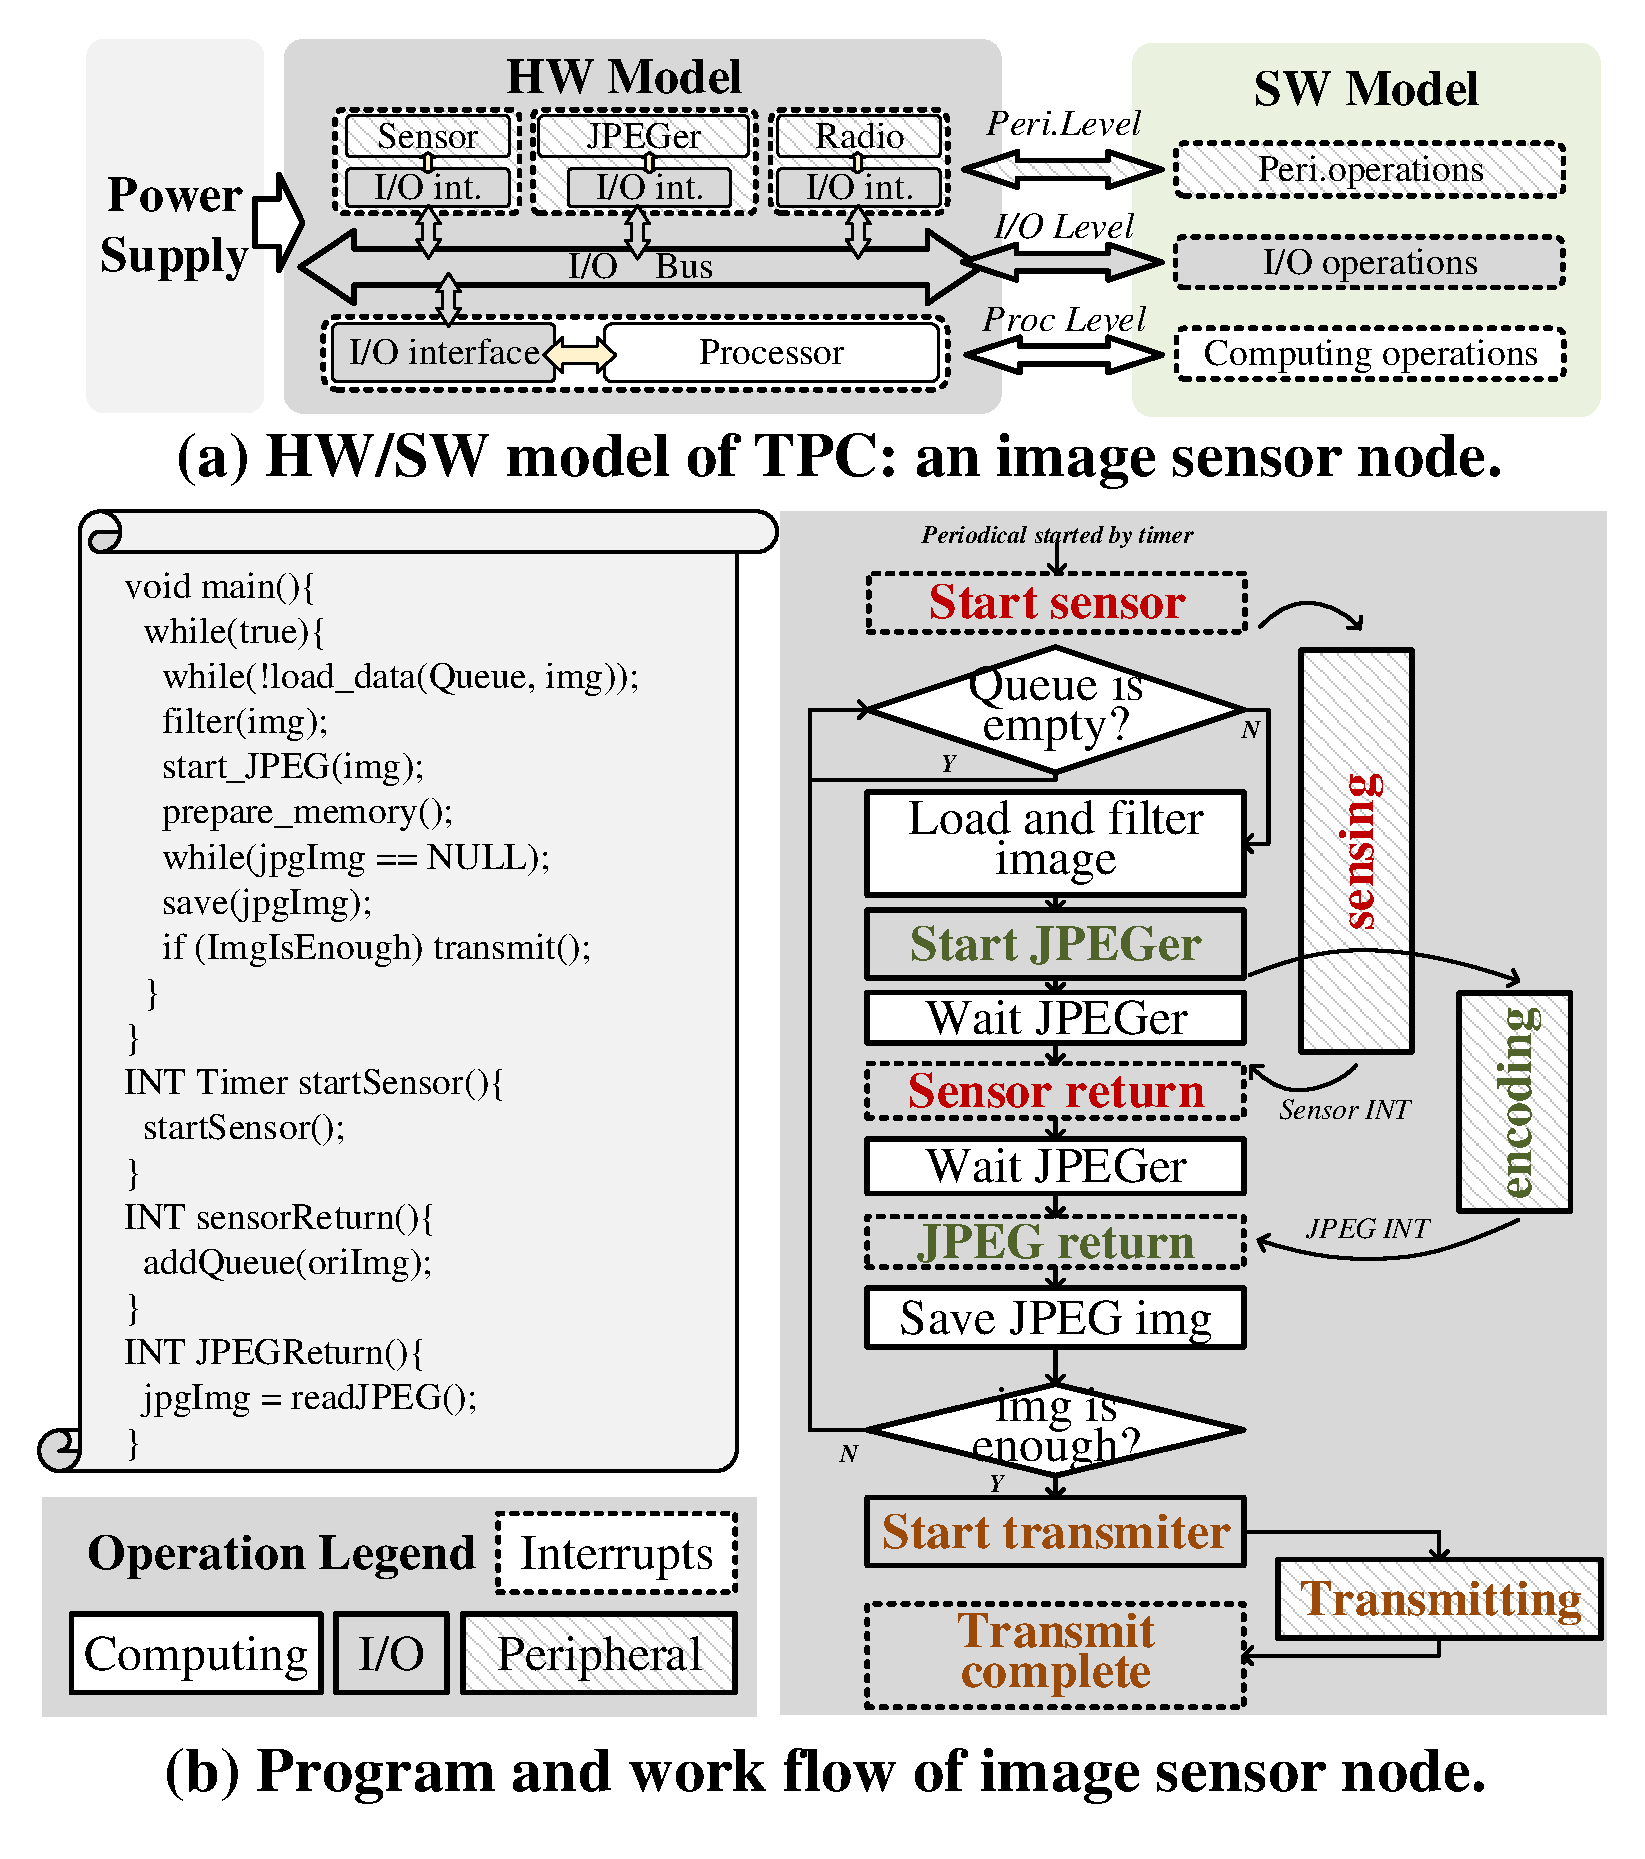
\includegraphics[width=0.47\textwidth]{Fig1_TPCModel.pdf}
    %\vspace{-10pt}
    \caption{An image sensing example used to present the HW/SW model of TPC system.}
    %\vspace{-5pt}
    \label{fig:TPCmodel}
\end{figure}

%\vspace{-5pt}
\subsection{TPC System Model} \label{sec:motiModel}
%\vspace{-5pt}
%
% Problem model and the requirements
Fig.~\ref{fig:TPCmodel} (a) exhibits the hardware structure of a typical TPC and the corresponding three types of operations on each hardware level. 
The sensor node contains a processor, multiple peripherals and the I/O bus to connect these hardware component.
The processor executes \emph{computing operations} and accesses the peripherals via \emph{I/O operations} on the I/O bus.
Peripherals, such as sensor, encoder and radio transceiver, are used to perform specific behaviors, such as sensing, data encoding and transmitting, with \emph{peripheral operations}.
These peripherals can be divided into three categories.
The input-type collects/receives the external information, such as a sensor or a touch screen.
The output-type realizes actuation to outside targets, such as a electromagnetic relay or a wireless transmitter.
The compute-type accelerates computing intensive tasks, such as a JPEG encoder.
Fig.~\ref{fig:TPCmodel} (b) shows the program model of a concurrent peripheral operation.
Before all, a peripheral should be completely initialized via I/O operations by the processor.
Then, the processor will write the start command to the peripheral, also via I/O operation, to start the actuation of the peripheral.
After that, the peripheral concurrently operates a specific peripheral operation and returns an interrupt to announce the processor when completed.
From this procedure, we can conclude that, (1) the peripherals requires more preparations to get ready; (2) I/O operations are atomic interacting operations between in the control thread of both processor and peripherals; (3) some peripheral operations are atomic, concurrent operations that only loaded on peripherals.

Fig.~\ref{fig:TPCmodel} (c) shows an image sensing example to explain the model.
The processor maintains two threads, the main thread and a timer thread. 
The timer thread periodically collects and stores the images into buffer.
In the main thread, the processor first initializes all the peripherals.
Then, in the loop of main thread, the processor processes and encodes the images with a JPEG encoder whenever the buffer is not empty.
When the process has stored enough encoded images, the sensor node will transmit all the images back to the server.
In this system, the image sensor is an input-type peripheral that collects outside images.
The radio transmitter is an output-type peripheral to transmit the collected images to the server for further processes.
The JPEGer is a compute-type peripheral to improve the computing performance and release the burden of the processor.

%
In intermittent power supply scenario, such a system can efficiently recover the processor and the computing operations with existed techniques. 
However, peripherals will lose their states after power failure, which leads to reliability and efficiency issues. 
Based on the type of peripherals, different faults will occur if the devices are not recovered: 
\textbf{1. Input-type Failure} may cause incompleteness and non-determinism. When a sensor loses power, the current collection will be crashed and result is non-deterministic. Even worse, one data lost may jeopardize the integrity of the whole data set in a multi-sensor system.
\textbf{2. Output-type Failure} may leads to large data loss and affect the application procedure. When the transmitter loses power, the current transmitting package as well as the data in peripheral buffer are lost. Moreover, the subsequent processes in the server are affect since none image arrives. Although costly software-level re-transmission can be used in some cases, it may not be feasible for resource-constraint energy-harvesting sensors. 
\textbf{3. Compute-type Failure} may cause fatal disruptions to the program. When the JPEGer loses power, processor cannot receive its returned results and halts all subsequent operations. It may cause system deadlock when program relies on the returned data.
Therefore, a systematical peripheral recovery mechanism is in desperate needs. 

Targeting on this requirement, two challenges arise.
(a) How to design an efficient architecture to recover the execution states in peripherals;
(b) How to devise a reliable checkpointing mechanism for a TPC with multiple peripherals.
The rest of this paper addresses these two challenges.

\subsection{Checkpointing for Concurrent TPC} \label{sec:motiSW}
%\vspace{-5pt}
%
Existing checkpointing strategy faces inefficient and reliability issues in recovering the TPC program where both non-atomic computing operations and atomic concurrent peripherals operations exist.

% static checkpointing
Static checkpointing strategy is safe for atomic operations but not efficient for non-atomic operations.
The red lines in Fig.~\ref{fig:motiRollback} (a) shows the efficiency issue caused by static checkpointing strategies~\cite{ransford2012mementos,Lucia2015,jayakumar2014quickrecall}.
Three execution threads are shown in the figure from top to bottom, that are the JPEGer thread, the sensor thread and the main thread of the processor.
The program presets checkpoints in position $cp1$, $cp2$ and $cp3$ to protect the atomic operations.
During execution, the program successively starts the sensor and the JPEGer.
Once power failure takes place during the I/O and peripheral operations, the program has to rollback to the complete safe position $cp1$ to restart all the devices which leads to extra waiting time and large rollback overheads.

% dynamic checkpointing
Dynamic checkpointing strategy is efficient for non-atomic computing operations on the processor but not safe for the atomic operations related to peripherals.
The blue lines in Fig.~\ref{fig:motiRollback} (a) shows the reliability issue caused by dynamic checkpointing strategies~\cite{wang20123us,liu2016a,Liu2015Ambient,balsamo2015hibernus}.
When power failure takes, the processor immediately place a checkpoint in position $cp4$.
From $cp4$, the main thread can efficiently continue with not rollback overhead, while all the peripheral devices are left un-recovered. 
Not only the disrupted peripheral operations failed, the peripherals are also left uninitialized which will leads to more errors when the subsequent peripheral-related operations are executed.

%
To realize both safe and efficient recovery, we need to combine the static and the dynamic checkpointing strategies for different operation types.
In Fig.~\ref{fig:motiRollback} (b), if the processor is restored to the interrupt position without rollback and all the peripherals are restarted from the static checkpoints before the atomic operations, the recovery overhead can be reduced by 58.5\%.
Therefore, an automatic checkpointing tool supporting a dynamic checkpointing strategy for TPCs with multiple peripheral is needed. 

%   
\begin{figure}[t]
    \centering
    \includegraphics[width=0.48\textwidth]{Fig1_motiRollback}
    %\vspace{-12pt}
    \caption{Challenges using static or dynamic checkpointing strategies in TPC. A hybrid checkpointing framework is needed.}
    %\vspace{-5pt}
    \label{fig:motiRollback}
\end{figure}

%%\vspace{-5pt}
\subsection{Hardware Needs for Peripheral Recovery} \label{sec:motiHW}
%\vspace{-5pt}
%
To support the hybrid checkpointing strategy, we still need hardware modifications based on existing hardware platforms.
Two drawbacks are noticed in the existing hardware platform shown in Fig.~\ref{fig:motiNVM} which contains a nonvolatile processor and sensors.

As is discussed above, NVP is the most efficient dynamic checkpointing strategy which is able to backup and restore (B/R) the processor state within $8\mu s$ once the supply voltage changes across the thresholds. 
However, both the B/R operations are passively triggered by the voltage detector.
NVP do not provide API to support the programmable backup operation for static checkpointing strategy.
Moreover, the processor may trigger unwillingly backup when power failure takes place during an atomic I/O operation in the main thread which will cause consistency problems. 
Therefore, it requires flexible B/R interfaces instead of the passive approach to support the hybrid checkpointing strategy.

% peripheral recover problem: restore and restart
On the other hand, checkpointing and recovering a peripheral also poses challenges.
Fig.~\ref{fig:motiNVM} shows the structure of an image sensor, a typical volatile peripheral.
The sensor contains a digital part using registers to store the states and data, and the analog part to realize the image collection operation.
When power failure takes place during a sensing task, the system has to not only restore the states in the register files, but also restart the analog part to re-execute the uncompleted sensing task to avoid the input-type failure.

\begin{figure}[t]
    \centering
    \includegraphics[width=0.48\textwidth]{Fig1_motiNVM}
    %\vspace{-15pt}
    \caption{Hardware challenges of multi-device checkpointing. NVP is limited by passive B/R function. Peripherals require efficient reconfigurations and restarts.}
    %\vspace{-5pt}
    \label{fig:motiNVM}
\end{figure}

To restore the states of the digital parts, existing approaches~\cite{jayakumar2014quickrecall,li2016hw} provides the 'load-and-backup' method.
To 'load-and-backup' with software methods, the processor has to read the internal registers in the sensor via I/O operations, which is energy hungry and time-consuming.
Moreover, as the number of peripherals increases, the recovery overhead becomes particularly significant.
% Any proof?
Li, et al.~\cite{li2016hw} provide hardware based solution by replacing peripheral registers to NVFFs which realizes efficient 'load-and-backup' procedure. 
But it requires hardware modifications inside the peripherals which is unrealistic considering the variety of peripheral types and producers.
Therefore, an efficient and general state restoring strategy is needed.
Furthermore, none existing strategy addresses the problem of restarting an uncompleted peripheral operations. 
Current systems can only rolling the entire system back to where the broken peripheral operations just started.
If a hardware module can simply re-execute the peripheral start program and return correctly, the peripheral restart can be more efficient.

Therefore, to efficiently and reliably recover concurrent TPCs, the enhanced NVP should support hybrid checkpointing, peripheral status monitor as well as the peripheral restart modules, which are all missing in existing NVPs.












\section{System Overview of REMARK} \label{sec:system}
%
To address the two challenges raised in Sec.~\ref{sec:motivation}, this paper proposes REMARK, an efficient and reliable multi-device checkpointing framework.
Fig.~\ref{fig:SystemArchitecture} shows the overview of REMARK framework, which contains an enhanced NVP architecture (Sec.~\ref{sec:hardware}), an offline program transformer (Sec.~\ref{sec:offline}) and an online recover procedure (Sec.~\ref{sec:online}).
The offline transformer pre-sets checkpoints to convert the original program to recoverable program for online execution.
The online recover procedure will adjust the checkpoints dynamically for further efficiency.
%And the hardware architecture provides efficient and flexible processor and peripheral checkpointing function interface.
The rest of this section presents the overview of each component.
The details will be covered in the rest of this paper. 

\vspace{5pt}
% hardware
\noindent\textbf{Enhanced NVP Hardware Support.} \\
As shown in Fig. 4, on top of existing NVP and NVIO that can instantly backup and restore the system state, REMARK adds four new modules to satisfy the requirements for flexible B/R functions and efficient peripheral recovery in the multi-device checkpointing strategy.

Two of these modules are used to help implement flexible and reliable processor checkpointing.
\textbf{B/R Manager} is designed based on the traditional B/R controller enabling both active and passive B/R operation.
Moreover, bootstrap is also added in this module to control the processor starting procedure.
\textbf{INT Recognizer (IRec)} is used to place safe checkpoint when power failure crashes a hardware interrupt where interactions between processor and peripherals locates.
The other two modules are used to realize efficient peripheral configuration and restart.
\textbf{Peripheral State Registers (PSRs)} is a real-time monitor of the peripheral state to support the efficient selective peripheral configuration.
\textbf{Peripheral Restart Module (PRM)} accelerates the peripheral restart procedure by automatically locating the start function in the program and correctly returning.
With the help of PRM, extra rollback of processor is removed.
To access these new modules, five new instructions are proposed as shown in Table~\ref{tab:InstrSet}.
Design details of the hardware architecture are presented in Sec.~\ref{sec:hardware} and Fig.~\ref{fig:HardwareArchitecture}.


\begin{figure*}[!htbp]
    \centering
    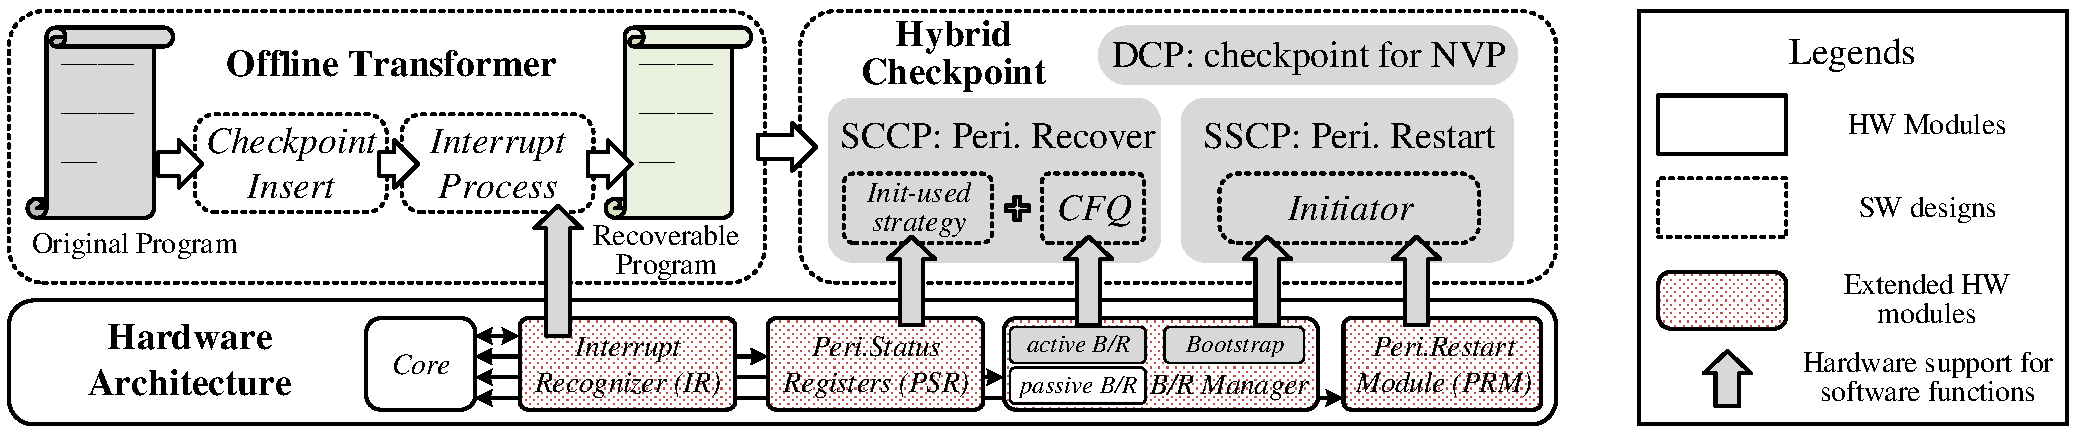
\includegraphics[width=1\textwidth]{Fig3_System.pdf}
    \caption{The HW/SW co-designed system diagram of REMARK.}
    \label{fig:SystemArchitecture}
\end{figure*}

%
\begin{figure*}[!htpb]
    \centering
    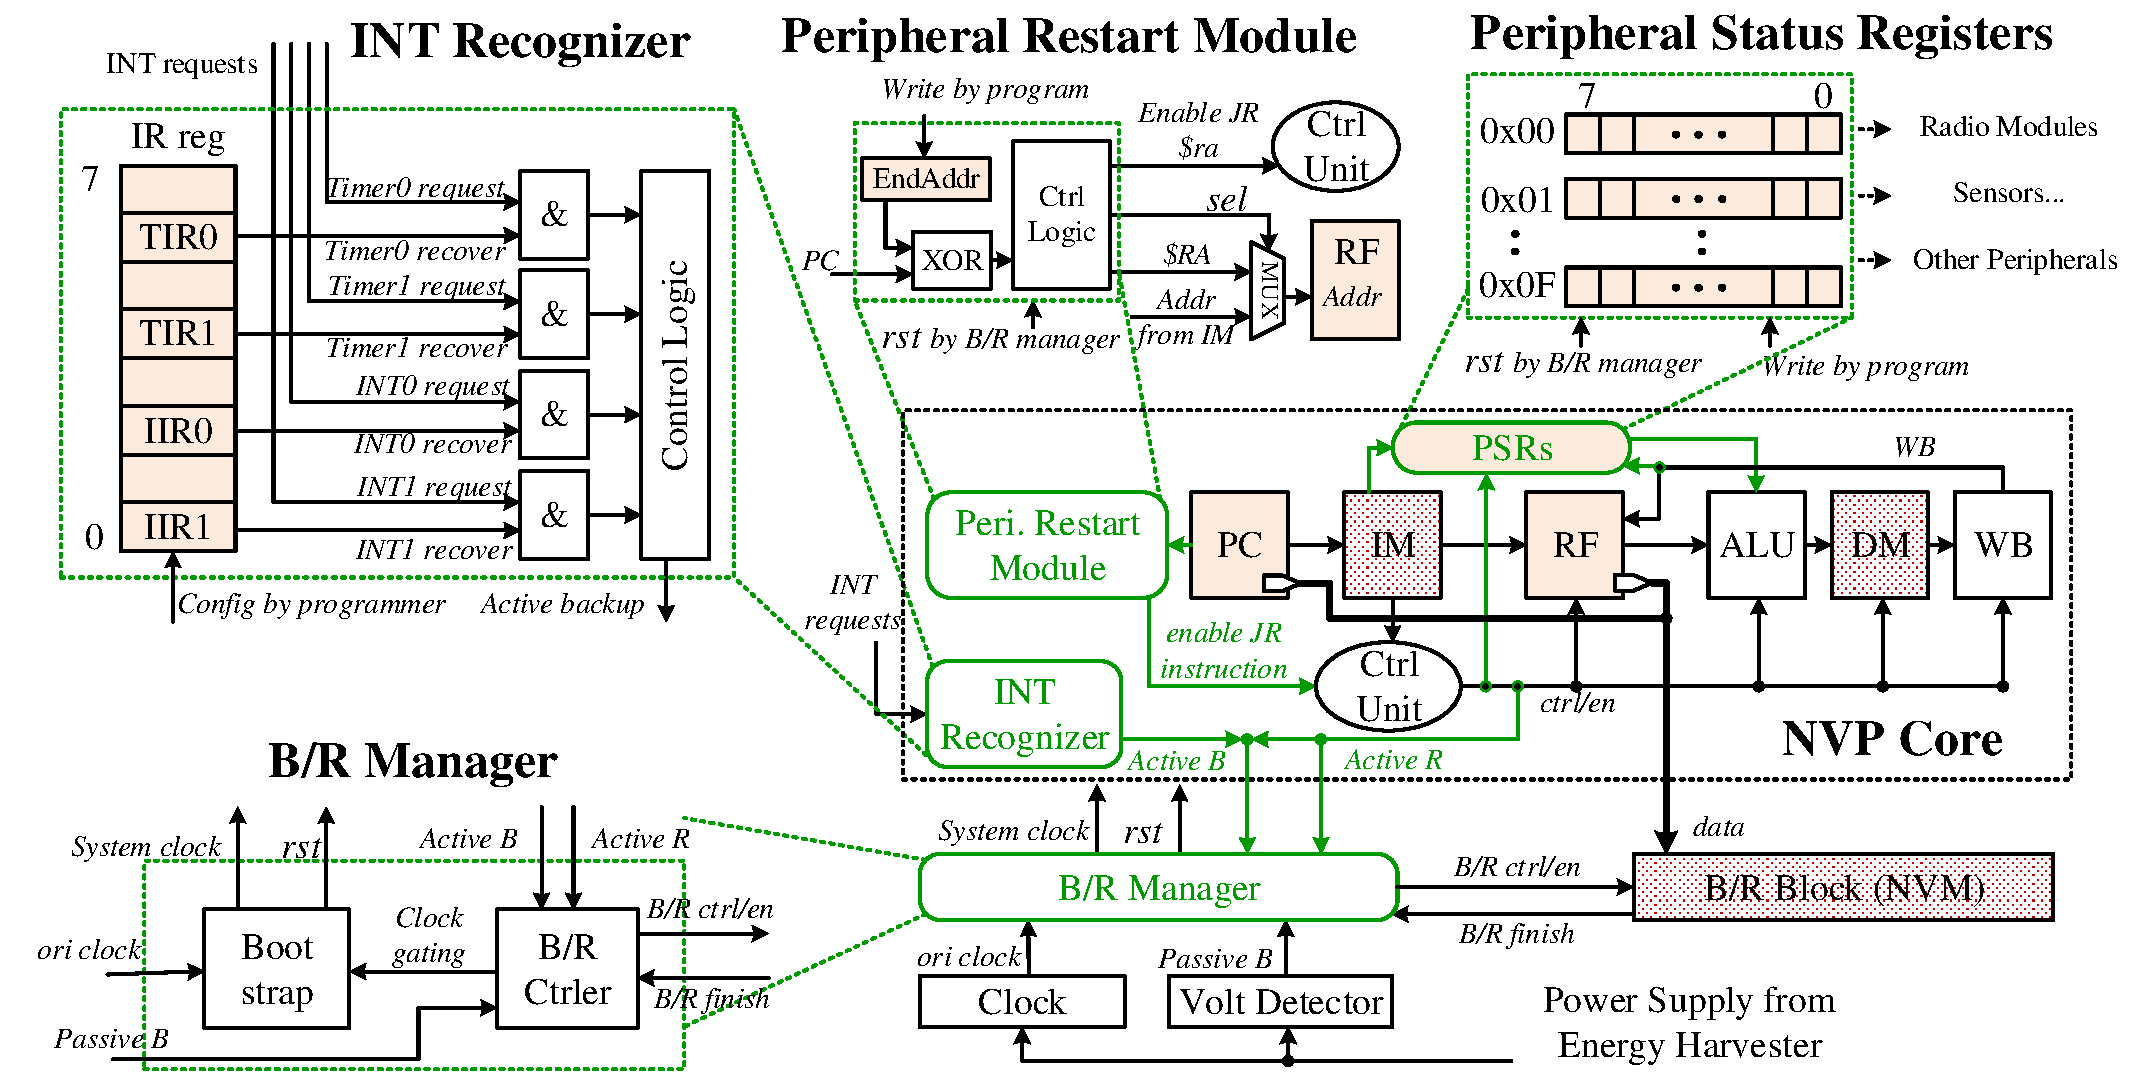
\includegraphics[width=1\textwidth]{Fig4_HardwareArchitecture.pdf}
    \caption{The hardware architecture of REMARK and its main modules. }
    \label{fig:HardwareArchitecture}
\end{figure*}

\begin{figure*}[!htbp]
    \centering
    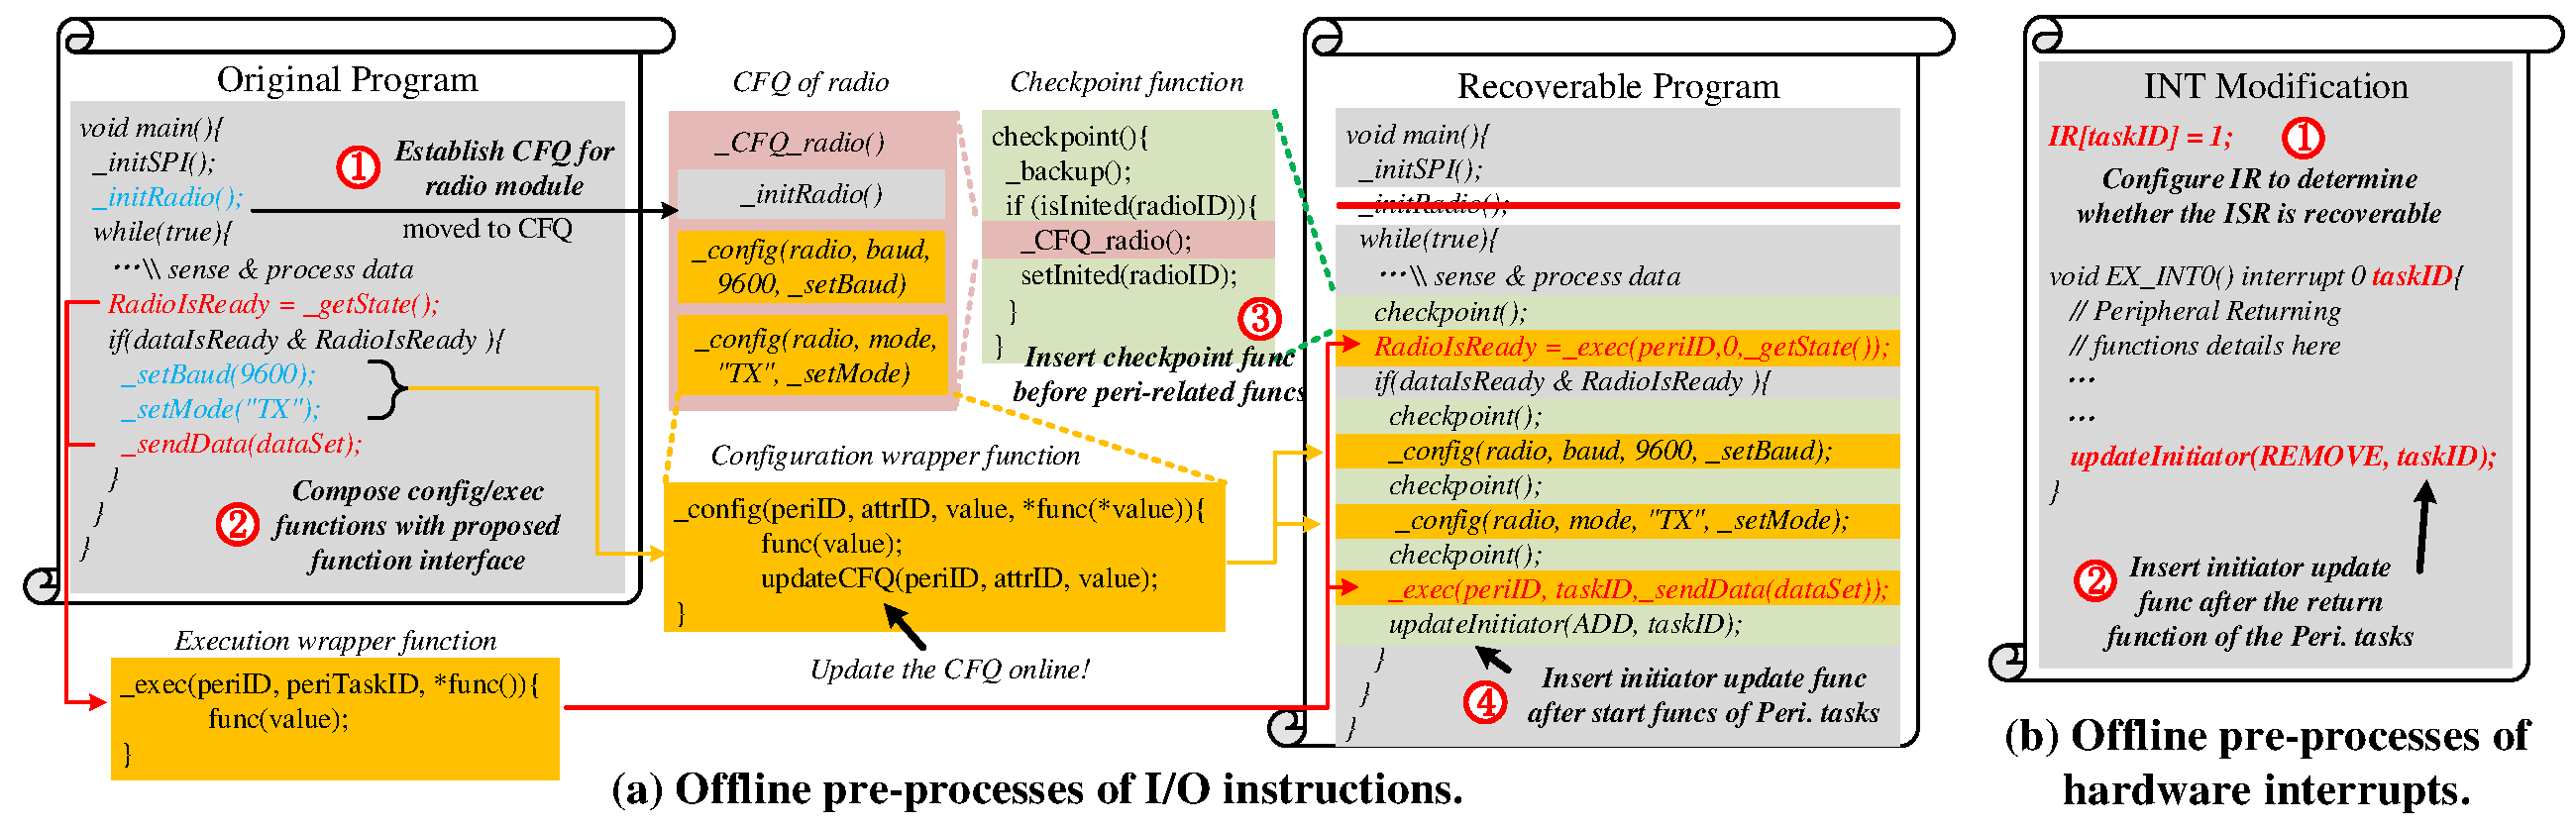
\includegraphics[width=1\textwidth]{Fig5_OfflineStage.pdf}
    \caption{The program pre-processes during the software transformation stage.}
    \label{fig:OfflineStage}
\end{figure*}

% offline
\vspace{5pt}
\noindent\textbf{Offline Program Transformer.} \\
REMARK addresses the multi-device checkpointing issue by pre-set the checkpoints according to checkpointing rules to ensure the recovery efficiency and reliability.
The transformer is used to transform the original program into recoverable program where reliable multi-device checkpoints are inserted.
The transformer first insert recoverable checkpoints by scanning the peripheral related operations.
Then the interrupts are processed to realize efficient and reliable interrupt recovery with the support of IR.
Details are presented in Sec.~\ref{sec:offline}.


% Online
\vspace{5pt}
\noindent\textbf{Online Recover Procedure.} \\
With the support of hardware architecture and the offline program transformer, an online recover procedure is proposed containing two parts, peripheral configuration and restart.
Based on PSRs, REMARK adopts an `init-used' strategy which only initializes and configures the invoked peripherals to avoid redundant reconfiguration overheads.
A config function queue (CFQ) is used to track and stores the peripheral configuration information.
The peripheral restart is realized by Initiator where peripheral checkpoints are stored.
Initiator is supported by the bootstrap in B/R Manager to control the system restart work flow.
After power failure, Initiator restarts all the checkpointed peripherals instantly and individually.
Considering the interactions of devices, the reliability of the entire recover procedure is guaranteed by the flexible B/R functions.
Details are explained in Sec.~\ref{sec:online}.

\begin{table}[t]
\caption{The extended instructions to the instruction set.}\label{tab:InstrSet}
\Fsize{8}
\renewcommand{\arraystretch}{1.5}
\begin{tabular}{cIcIm{4.4cm}}
    \Xhline{1.2pt}
    Instructions       & Operators           & Specifications      \\
    \Xhline{1pt}
    RSR      & SRaddr   oper2 & Read PSRs with address \emph{SRaddr} to register \emph{oper2}.\\
    \Xhline{1pt}
    WSR     & oper1   SRaddr & Write the value of \emph{oper1} to PSRs with address \emph{SRaddr}.\\
    \Xhline{1pt}
    WER    & oper1               & Write the value of \emph{oper1} to \emph{EndAddr} register in PRM.\\
    \Xhline{1pt}
    ABR     & oper1               & Enable the active backup function, if $oper1=1$; enable the active restore function, if $oper2=0$.\\
    \Xhline{1pt}
    EBR     & oper1               & Enable/Disable the backup and restore function when $oper1=1/oper1=0$.\\
    \Xhline{1.2pt}
\end{tabular}
\end{table}



\section{Enhanced NVP Architecture} \label{sec:hardware}
%\vspace{-5pt}
%
To impletement REMARK, NVP is enhanced by four hardware modules to support flexible B/R functions and realize efficient peripheral recovery.

\vspace{5pt}
\noindent\textbf{Backup/Restore (B/R) Manager.} \\
Existing NVP only supports passive B/R functions, which limits the flexibility of NVP.
Passive backup operation can only be triggered when the supply voltage is below the threshold.
When power recovers, passive restore operation is activated automatically and no initiator program is allowed. 
Target on these challenges, B/R Manager extends active B/R functions to support flexible checkpointing.
Moreover, a Bootstrap module is also added to support the initiator program.
The structure of the B/R Manager is shown in Fig.~\ref{fig:HardwareArchitecture}.

%
The B/R controller is enhanced by control logics which are used to select the trigger signal of B/R functions.
Two instructions, \emph{ABR} and \emph{EBR} (Table~\ref{tab:InstrSet}), are added to enable the active B/R functions.
Active backup is realized by \emph{ABR 1}, and active restore is \emph{ABR 0}.
In addition, \emph{EBR 0} and \emph{EBR 1} are used to disable and enable the B/R function, respectively.

%
Bootstrap is a module used to control the system clock and the reset signals.
Its work flow is shown in Fig.~\ref{fig:InitiatorFlow}.
After the system is powered on, Bootstrap selects whether to enter the restart procedure or to start the program from the very beginning according to the \emph{$1^{st}\_start$} signal.
\emph{$1^{st}\_start$} is an external signal set by users.
If \emph{$1^{st}\_start$} is set, the processor is started from the very beginning.
Otherwise, Initiator is started to recover the peripherals and restore the processor.
%Bootstrap generates the system clock for the processor and resets the modules before the entire system starts.
%Bootstrap can also gate the system clock when an active backup function is invoked.

%
\begin{figure}[t]
    \centering
    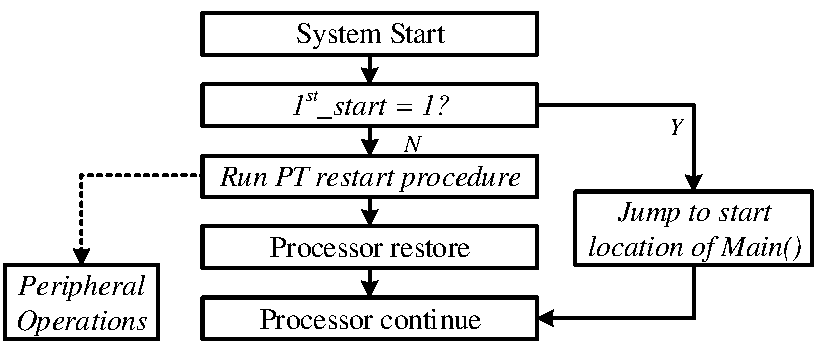
\includegraphics[width=0.48\textwidth]{Fig9_InitiatorFlow.pdf}
    \vspace{-10pt}
    \caption{The flow chart of Initiator.}
    \label{fig:InitiatorFlow}
\end{figure}

\vspace{5pt}
\noindent\textbf{Interrupt Recognizer (IRec).} \\
%
Interrupt is an interaction between processor and the peripherals where careful checkpoints should be placed.
IRec provides hardware support for reliable interrupt recovery.
It recognizes the interrupt request and decides whether to recover the interrupt.
Fig.~\ref{fig:HardwareArchitecture} shows the hardware diagram of this module.
Firstly, IRec contains a nonvolatile special register to store a programmable control bit, IR, which indicates whether an interrupt is recoverable.
If the interrupt is recoverable, IR is set and the system will recover the interrupt as a normal processor task.
Otherwise, IR is reset.
When an unrecoverable interrupt request arrives, the control logic triggers B/R Manager to execute a backup operation and set a checkpoint before the interrupt.
In this way, the system will resume from the checkpoint and skip the interrupt after power failure.

\vspace{5pt}
\noindent\textbf{Peripheral Status Registers {(PSRs)}.} \\
PSRs are used to monitor the peripheral status in real-time to support efficient peripheral reconfiguration.
PSRs in Fig.~\ref{fig:HardwareArchitecture} is a group registers, each bit of which indicates whether a peripheral is ready or not.
These states will be set when the peripherals are configured and cleared after power failures.
Thus, a group of volatile registers are the ideal choice.
Since the internal registers are all non-volatile and are resumed after power failures, PSRs are added as external registers.
%When the system recovers after power failures, PSRs will be reset by the reset signal generated by the B/R Manager.

PSRs can be accessed by the processor with the proposed instruction \emph{RSR} and \emph{WSR} as shown in Table~\ref{tab:InstrSet}.
\emph{RSR} reads the value from \emph{SRaddr} into the register \emph{oper2}.
\emph{SRaddr} is the address of PSRs and has an independent address space from the register file.
\emph{oper2} can be the address of a normal register, a direct address or an indirect address.
Similarly, \emph{WSR} writes the value of second operand \emph{oper1} into \emph{SRaddr}.
\emph{oper1} can be the address of a normal register, a direct address, an indirect address or an immediate operand.

\vspace{5pt}
\noindent\textbf{Peripheral Restart Module (PRM).} \\
PRM is used to locate the start function of peripherals and realize correct returning during the restarting procedure.
As shown in Fig.~\ref{fig:HardwareArchitecture}, PRM contains a special register \emph{EndAddr}, an XOR gate and the control logic.
When a peripheral needs to be restarted, PRM is called by the processor with two instructions.
Firstly, the end address of the peripheral start function is stored to \emph{EndAddr}.
Then, the program jumps to the peripheral start function with a \emph{JAL} instruction.
When the program counter reaches the end address, the XOR gate generates a positive trigger and the control logic enables a \emph{JR \$ra} instruction automatically.
In this way, the peripheral is successfully restarted and the program returns correctly to restart the next peripheral.
%\vspace{-5pt}
\section{Multi-deivce Checkpointing} \label{sec:offline}
%\vspace{-5pt}
%
With the enhanced NVP, REMARK will process the original program with the offline program transformer to pre-set safe checkpoints to collaborate with the new hardware modules to ensure correct online execution.

%\vspace{-5pt}
\subsection{Checkpoint Rules for Multi-device TPC}\label{sec:offlineRules}
\vspace{-5pt}
%
In multi-device systems, we should realize reliable checkpoints considering the processor, the peripherals and the interactions between devices.

As discussed above, a peripheral cannot keep its state when it is interacting with the processor or the environment.
Therefore, \emph{the peripheral checkpoints can only be placed when the peripheral is idle.}
For example, \emph{cp1} and \emph{cp2} in Fig.~\ref{fig:InteractDefine} are two available checkpoints to store the state of the sensor.

In contrast, NVP allows checkpoints at any position in the program and can recover safely.
However, the interaction between processor and peripherals may cause inconsistency.
When power fails during these interactions, the processor may keep its state while the peripheral needs to roll back to a previous position, which leads to inconsistency.
Therefore, \emph{the processor checkpoint should be placed out of the processor-peripheral interaction operations.}

Fig.~\ref{fig:InteractDefine} shows two types of processor-peripheral interactions: I/O operations and interrupts.
First type is I/O operations started by processor to write configurations or commands to peripherals.
Here, if power fails when the processor is configuring or starting the sensor, the processor should rollback to \emph{cp1} or \emph{cp2} to restart the I/O operation.
Second type is the external interrupt activated by peripherals.
Sensor triggers an interrupt when the sensing task is completed, then, the processor read the operation result from the sensor.
If power failure occurs during an interrupt, the processor should not recover the interrupt service routine (ISR).
Instead, it should rollback to \emph{cp3}, the entrance before the interrupt in the main process.
In this way, when the power resumes, ISR is skipped to avoid processing corrupted data in ISR.

Based on these rules, the offline program transformer scans the whole program and inserts safe checkpoints according to the positions of the I/O instructions and the interrupts.

%   
\begin{figure}[t]
    \centering
    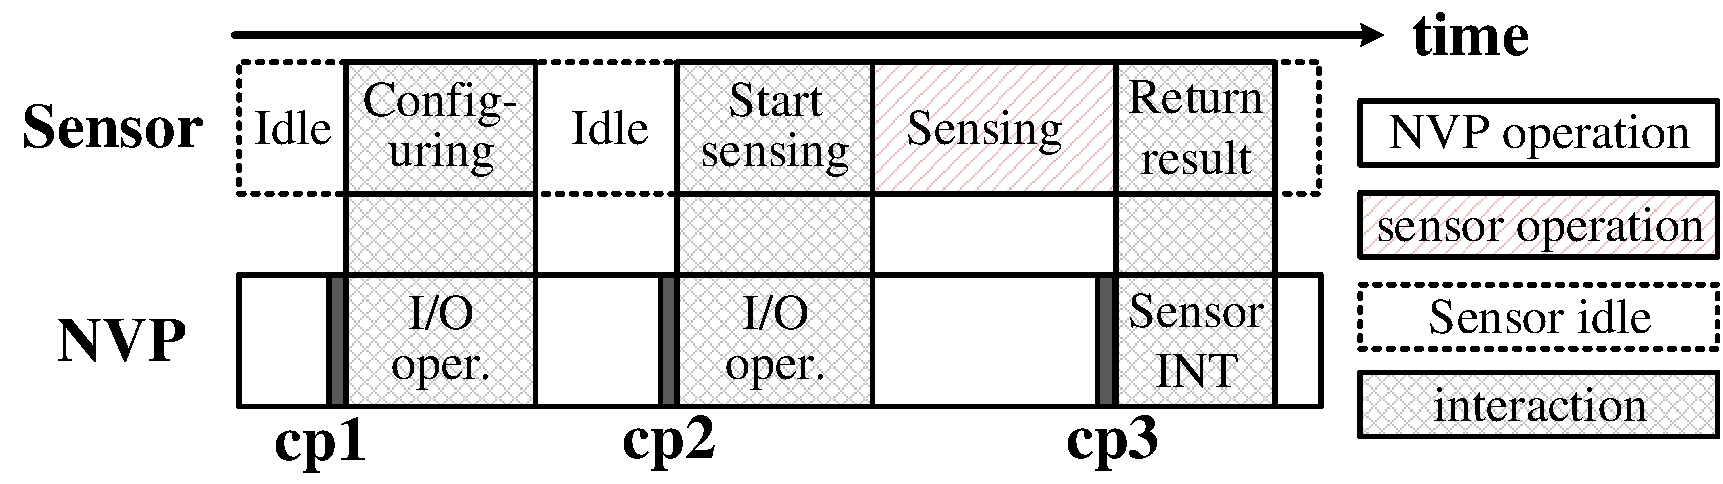
\includegraphics[width=0.48\textwidth]{Fig7_InteractDefine}
    \vspace{-15pt}
    \caption{Interactions between processor and peripheral.}
    \vspace{-5pt}
    \label{fig:InteractDefine}
\end{figure}


\subsection{Offline Program Transformer} \label{sec:offlineTransformer}
\vspace{-5pt}
The offline program transformer contains two steps to handle the I/O instrucitons and the hardware interrupts.

%
\vspace{5pt}
\noindent\textbf{Handle I/O Instructions.} \\
REMARK categorizes I/O instructions into two groups: peripheral configuration instructions and peripheral execution instructions. 
Configuration instructions, including the initialization instructions, are used to configure the internal registers of peripherals.
Execution instructions are used to realize the functionalities of peripherals, such as starting a communication, fetching data from a peripheral buffer, etc. 
Before execution instructions, configuration instructions are required to set the peripherals ready.

%
The pre-processing for I/O instructions involves three steps. 
Fig.~\ref{fig:OfflineStage} shows a data transmission example to illustrate the procedure.
Firstly, REMARK establishes a configuration instruction queue (CFQ) for each peripheral. 
CFQ tracks configuration instructions, including the initialization instructions, of a peripheral, which are used to configure the peripheral in case of power failures.
Every time a new configuration instruction is executed, CFQ will be updated to include the latest configuration modification.

%
To allow REMARK to recognize and pre-process the I/O instructions, the programmers have to implement the peripheral configuration and execution instructions with wrapper functions indicated in the orange parts of Fig.~\ref{fig:OfflineStage}. 
Here, the configuration wrapper function contains the peripheral ID, the target attribute, the configuration value and the pointer of the configuration instruction.
It will execute the configuration instructions and update CFQ with function \emph{\_updateCFQ()}, which will be described in Sec.~\ref{sec:online}.
Execution wrapper function contains the peripheral ID, the peripheral operation ID and the target instruction pointer.
A non-zero peripheral operation ID represents that the instruction starts a peripheral operation.

%
After peripheral related instructions are recognized, two recovering functions are inserted into the program to set checkpoints of processor and peripherals. 
Firstly, a \textbf{checkpoint function} is inserted before each I/O instruction to checkpoint the processor.
With the checkpoint function, the processor rolls back to reconfigure the peripherals to avoid inconsistency.
Second, \textbf{initiator update functions}, \emph{updateInitiator()}, are inserted after the execution instructions of peripheral operations to set peripheral checkpoints.
\emph{updateInitiator(ADD, taskID)} records the start position and the end position of the start program of the peripheral operations, \emph{PT(taskID)}, and adds its peripheral checkpoint into Initiator.
These checkpoints are used to restart the crashed peripheral operations.
Circle 3 and 4 in Fig.~\ref{fig:OfflineStage} (a) illustrates these two functions.
%The details of these two instructions are explained with the recover procedures in Sec.~\ref{sec:online}.

%
\vspace{5pt}
\noindent\textbf{Handle Hardware Interrupts.} \\
Fig.~\ref{fig:OfflineStage} (b) shows the ISR processing procedure with two steps. 
The first step is to set safe checkpoints considering the consistency of processor-peripheral interactions.
Generally, an ISR should not be recovered, if it contains processor-peripheral interactions.
Consider the case that, the embedded volatile memory in a sensor loses all the data after power failure.
If the processor resumes the ISR, it will receive wrong data from the sensor which leads to system errors.
However, ISRs which contain no interactions can be safely recovered after power failure, such as a counter triggered by a timer.
To solve this application specific issue, REMARK provides a control bit, \emph{IR}, to the application developers to indicate whether an ISR can be restored according to application requirements.
Programmers can reset IR, if an ISR is recoverable, or set IR, if it's unrecoverable.
The IR is stored in IRec and the latter can set reliable checkpoints automatically during execution.

The second step is to maintain the peripheral checkpoints.
An interrupt started by a peripheral indicates that the peripheral has completed its task and will enter idle mode.
The system does not need to restart a task if power fails after its completion.
To remove such invalid checkpoint, Initiator update function is inserted at the end of each ISR.
\emph{updateInitiator(REMOVE, taskID)} removes the peripheral checkpoint of \emph{PT(taskID)}.

%
In this way, the program is transformed to be recoverable.
It is now ready to realize recoveries on the proposed hardware. 
Noted that, \emph{programmers can dictate an operation as unrecoverable by not using the wrapper codes according to application-specific reasons, such as data freshness requirements}.

\begin{comment}
\textbf{Optional Recovery Approach}
%
In our design, the integrated master interface of an I/O bus is a non-volatile I/O interface, which utilizes NVFFs to re-initialize and re-configure the I/O bus~\cite{li2016hw}.
No hardware modification is required for the external peripherals. 
The recovery of the operations is optional via software approaches. 
To avoid recovering an operation, the \emph{periTaskID} in the wrapper function as well as the related IR bit is set to zero.

%
The recovery of tasks is application specific and defined by programmers.
However, two kinds of applications are recommended to be recovered to confirm the reliability and achieve higher data acquisition.
First is the applications that rely on hardware interrupts.
Recovering these applications can avoid deadlock caused by un-returned interrupts. 
Second is the normally-off applications requiring frequent 'OFF-ON' switching. 
REMARK realizes fast re-initialization which can improve the data acquisition for long-term periodical data collections.
\end{comment}
\section{Online Recover Procedure} \label{sec:online}
%
With the support of hardware architecture and offline program transformer, this section presents the online recover procedure, including the reconfiguration (Sec.~\ref{sec:onlineReconfig}) and the restart (Sec.~\ref{sec:onlineRestart}) of peripherals.






\subsection{Peripheral Operation Restart} \label{sec:onlineRestart}
%\vspace{-5pt}
%
After the peripherals are reconfigured, we are ready to restart the peripheral operations.
REMARK restarts the peripheral operations from peripheral checkpoints with the help of PRM (described in Sec.~\ref{sec:hardware}) and Initiator.



%\vspace{5pt}
\noindent\textbf{The Restart Flows after Power Failure.} \\
The restart flows are different from each other when power fails during different stages.
A peripheral operation can be decomposed into three stages: the starting stage, the execution stage, and the returning stage.
During the starting stage, the processor uses I/O instructions to start a peripheral operation.
The execution stage lasts until the returning interrupt is triggered.
Finally, the ISR returns the result to the processor in the returning stage.
The peripheral operation is completed only if the ISR is finished.

%
When power fails during the starting stage, the parallel peripheral operation has not been started.
No peripheral checkpoints are placed, and the processor only needs to rollback and re-run the starting stage.
Once the starting stage is completed, \emph{updateInitiator()} inserted during offline program transformation will place a peripheral checkpoint in Initiator.

When power fails during the execution stage, as shown in Fig.~\ref{fig:PeriRecoverProcedure} (a), the processor restores its state and the peripheral operations are restarted from their checkpoints individually.

When power fails during the returning stage, as shown in Fig.~\ref{fig:PeriRecoverProcedure} (b), the peripherals lose all the data and fail to return the results.
Therefore, the peripheral operations still need to be restarted.
Meanwhile, the processor needs to restore to the checkpoint located before the ISR, as discussed in Sec.~\ref{sec:offlineTransformer}.
When a successful ISR is completed, the peripheral operation is also finished.
Therefore, the peripheral checkpoint to restart this operation needs to be removed from Initiator by another \emph{\_updateInitiator()} function.

%
\begin{figure}[t]
    \centering
    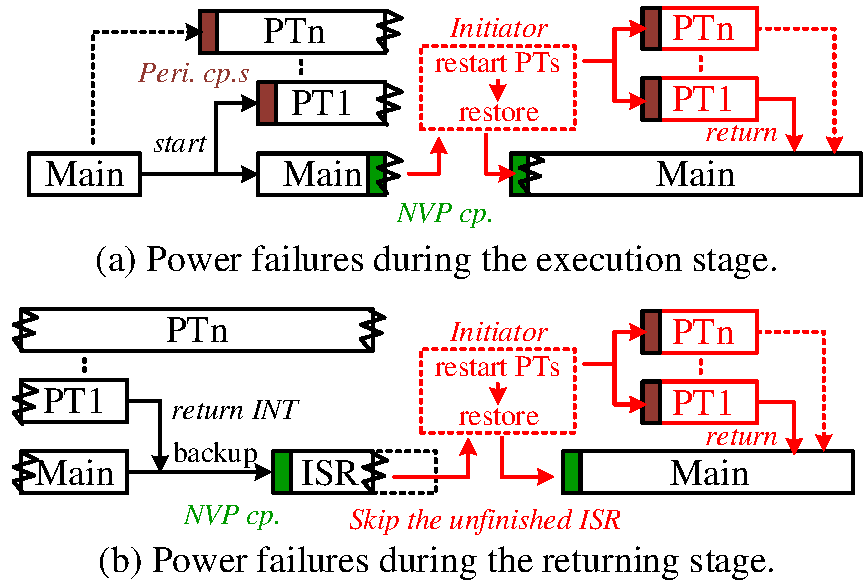
\includegraphics[width=0.45\textwidth]{Fig10_PeriRecoverProcedure.pdf}
    %\vspace{-5pt}
    \caption{Power failures during the starting and the returning stage of peripheral operations.}
    %\vspace{-5pt}
    \label{fig:PeriRecoverProcedure}
\end{figure}

% the resilience of REMARK
When power fails during the recover procedure, the devices can roll back to their checkpoints if these checkpoints are not crashed.
Therefore, completing the backup function is essential to ensure the validity of a checkpoint.
To guarantee the success of backup operation, NVP adopts a $4.7 \mu F$ on-chip capacitor.
In the hardware prototype of this paper, each backup operation consumes $77.69nJ$ in $7 \mu s$.
In this way, the system can safely backup whenever power fails.

\section{Hardware Implementation} \label{sec:implementation}
%\vspace{-5pt}
%
In order to evaluate the performance and resiliency, we implements REMARK on an Intel 8051 based NVP as well as a hardware platform, \emph{NVnode}.
In this section, we first present the hardware platform in Sec.~\ref{sec:implHW}. 
Then, the improvement of the peripheral recovery and the overall performance are presented in Sec.~\ref{sec:implPeriRecover} and Sec.~\ref{sec:implOverall}, respectively. 

\subsection{Hardware Platform} \label{sec:implHW}
%\vspace{-5pt}
%NVP
Fig.~\ref{fig:NVnode} shows a picture of NVP chip and NVnode platform.
The structure of NVnode is presented in Fig.~\ref{fig:ImpNVRF}.
NVnode contains a power supply system, an NVP with proposed REMARK modules and peripherals including ZigBee transceiver and sensors.
The energy storage is a $20\mu F$ capacitor which is charged between $1.2V$ and $5V$.
The total storage of the capacitor is $212\mu J$ while the energy efficiency is $90\%$.

% NVP
The parameters of the proposed NVP are listed in Table.~\ref{tab:NVnodePara}.
This NVP is designed based on Intel 8051 ISA. 
It contains a $256B$ register file using NVFF, a $32KB$ FeRAM data memory, a B/R Manager and an NVRF module to enable REMARK.

% NVRF
As shown in Fig.~\ref{fig:ImpNVRF}, NVRF realizes the functionality of PSRs and PRM, which enable efficient and reliable peripheral configuration and restart operations.
NVRF contains a $32B$ register file, an RF controller, and an SPI interface.
The register file stores the state of the wireless transceiver.
The RF controller can reconfigure the transceiver and restart the data transmission task automatically and efficiently after power failure.
The SPI interface is used to mount to SPI bus, which also connect to a ZigBee transceiver and several sensors.

%
\begin{figure}[t]
    \centering
    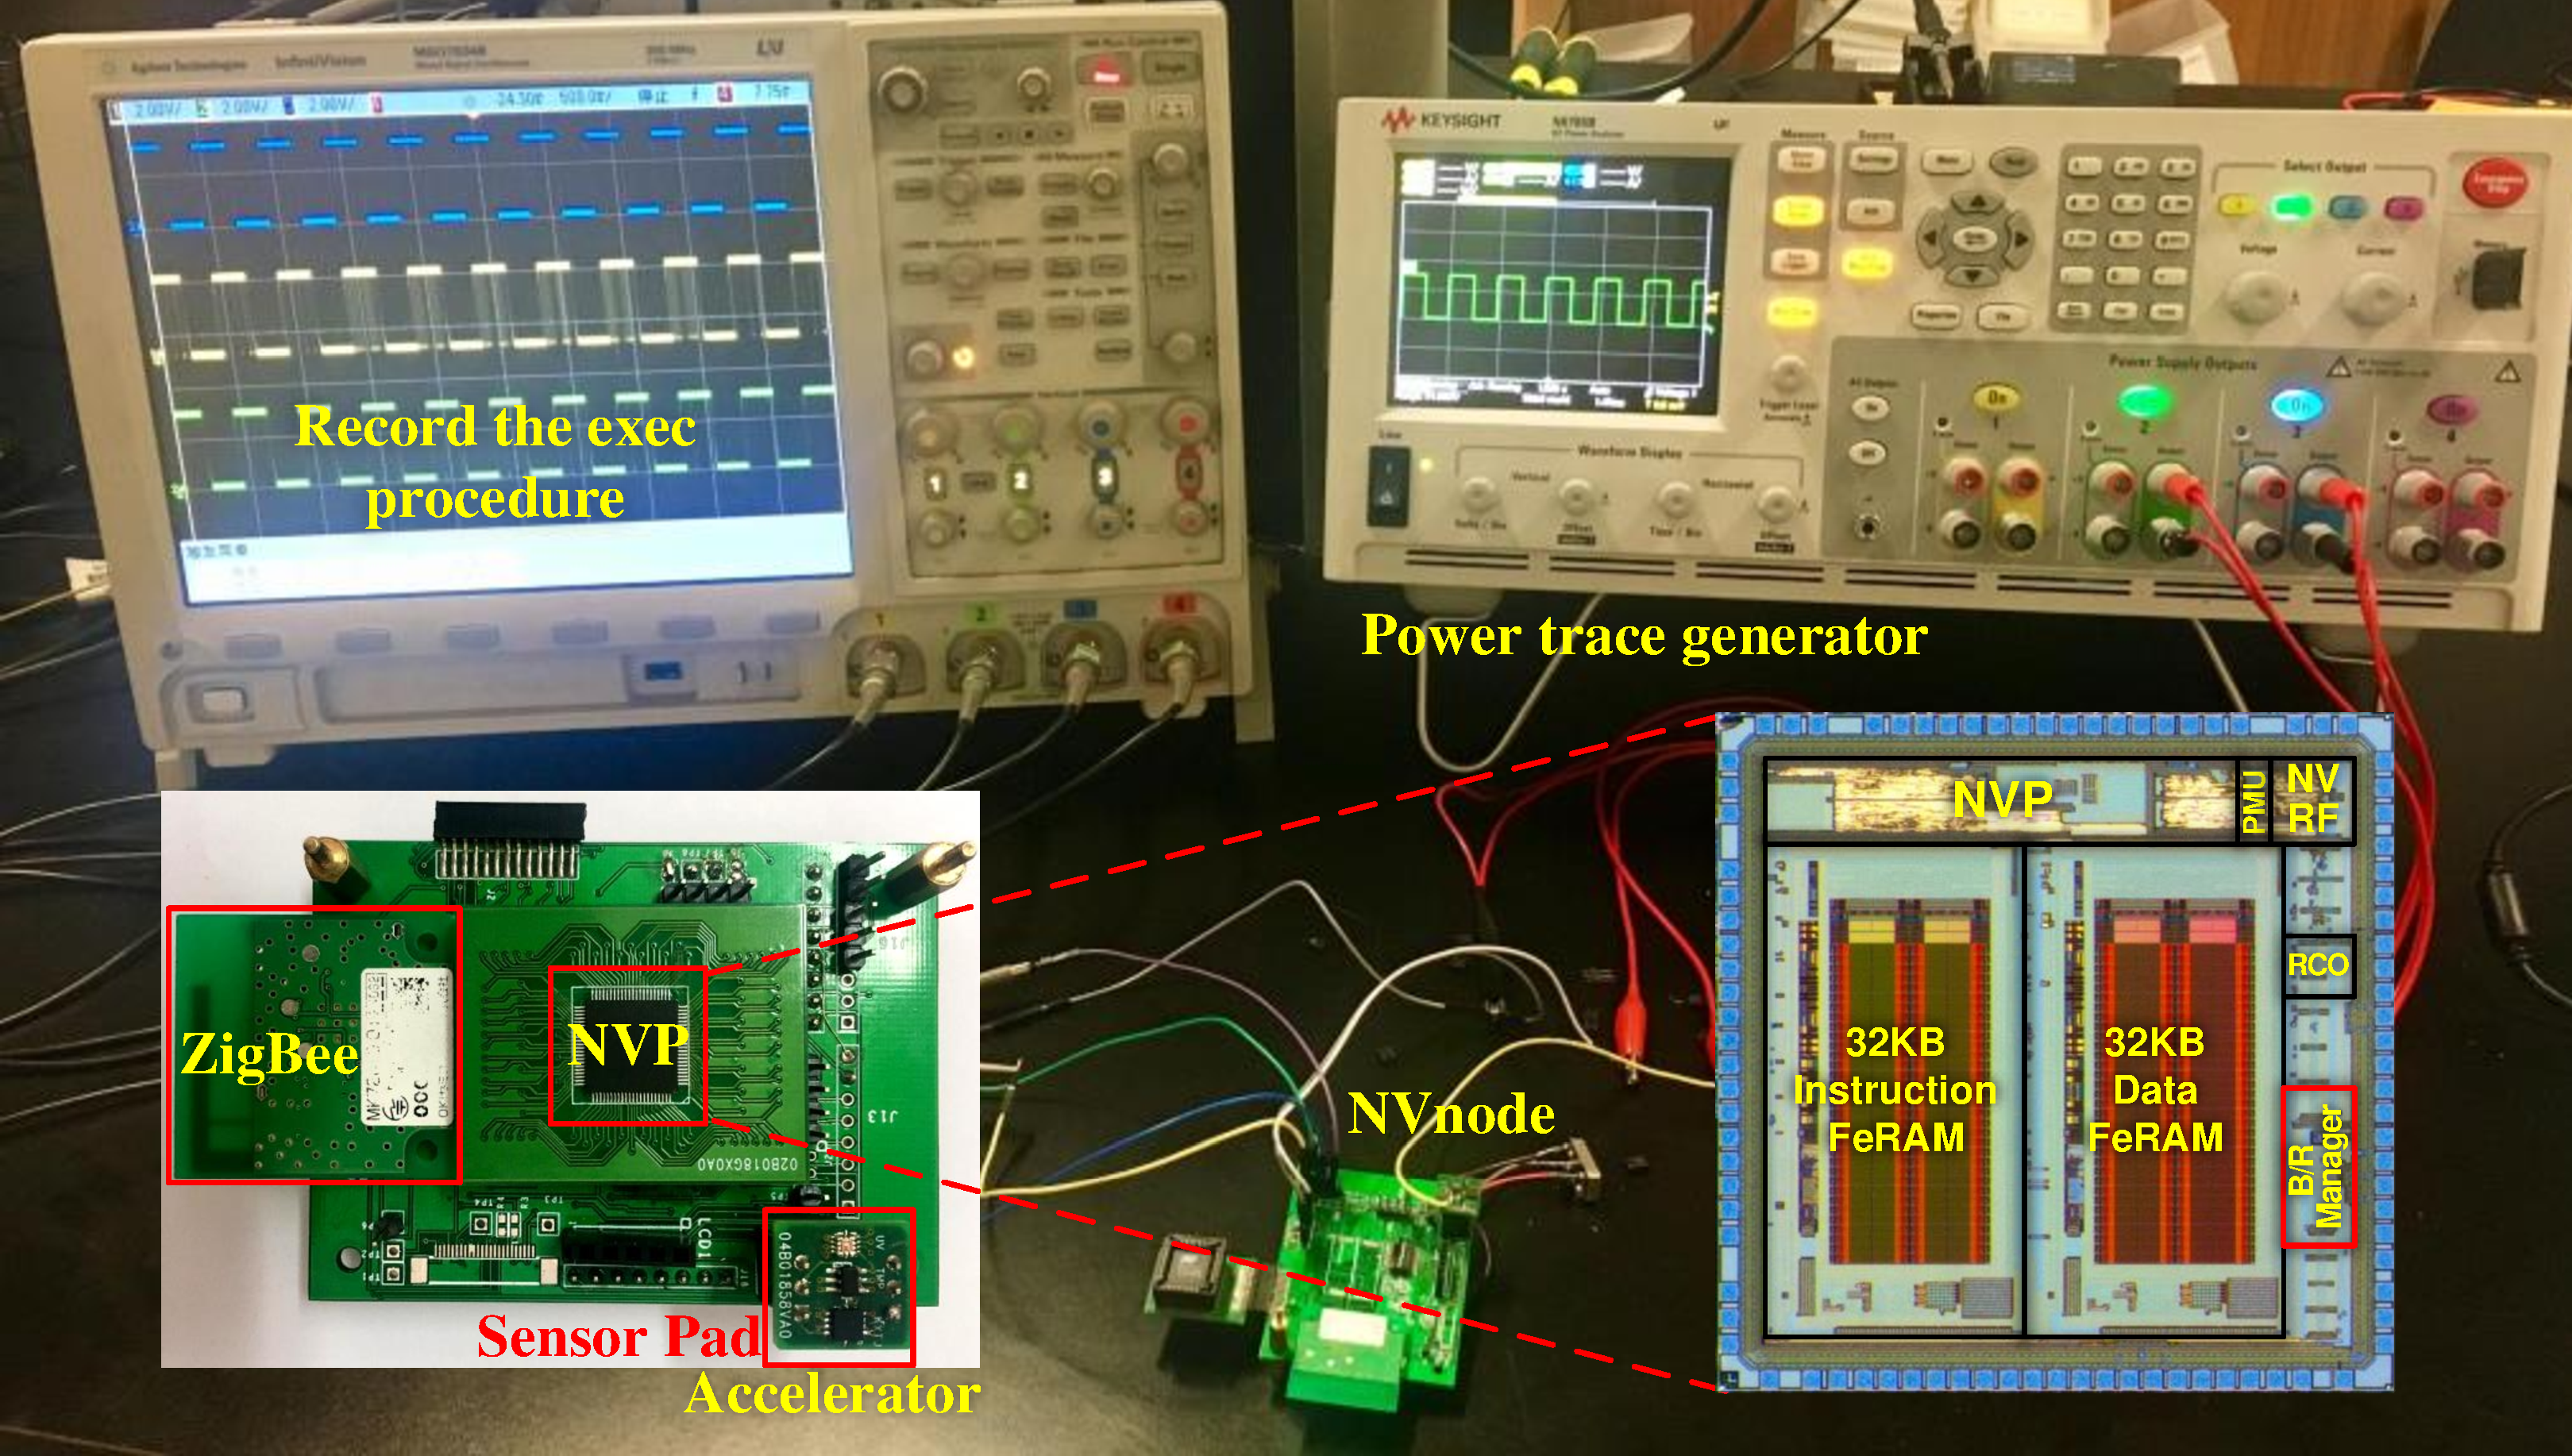
\includegraphics[width=0.48\textwidth]{Fig11_NVnode.pdf}
    %\vspace{-10pt}
    \caption{The hardware platform, NVnode. REMARK is implemented with the B/R manager and the NVRF controller in an 8051 NVP chip under $0.13\mu m$ technology.}
    %\vspace{-5pt}
    \label{fig:NVnode}
\end{figure}

\begin{figure}[htpb]
    \centering
    %\vspace{-0pt}
    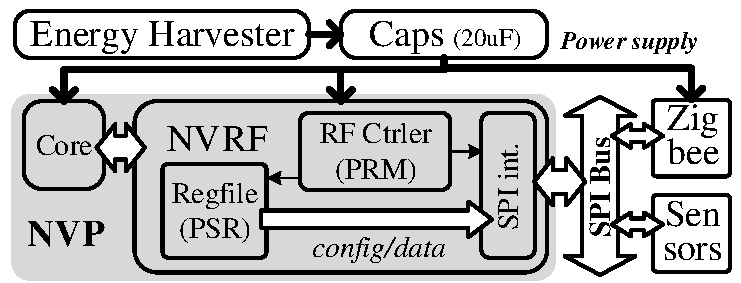
\includegraphics[width=0.4\textwidth]{Fig11_ImpNVRF.pdf}
    %\vspace{-2pt}
    \caption{The structure of NVnode. The energy storage is $20\mu F$. NVRF implements the functionality of PSRs and PRM to accelerate the peripheral recovery.}
    %\vspace{-5pt}
    \label{fig:ImpNVRF}
\end{figure}

\begin{table}[t]
\begin{center}
\vspace{-0pt}
\caption{The parameters of NVP.} \label{tab:NVnodePara}
\vspace{-5pt}
\Fsize{8}
\renewcommand{\arraystretch}{1.5}
%\setlength{\tabcolsep}{1pt}
\begin{tabular}{Ic|cIc|cI}
    \Xhline{1.2pt}
    Parameter                        & Value                    & Parameter                    & Value        \\
    \Xhline{1pt}
    Process Technology        & $0.13\mu m$         & Clock frequency           & $1MHz$        \\
    %\Xhline{1pt}
    %TMP Sensor                    & TMP100               & RF Module                   & ML7266    \\
    \Xhline{1pt}
    Backup Time                  & $5\mu s$               & Restore Time                & $3\mu s$   \\
    \Xhline{1.2pt}
\end{tabular}
\vspace{-15pt}
\end{center}
\end{table} 

\subsection{Device Recovery Improvement of REMARK} \label{sec:implPeriRecover}
%\vspace{-5pt}
%
To show the effectiveness of REMARK, this subsection first shows the overhead reduction of a single transceiver recovery. 
Then, it shows the efficiency improvement when there are multiple peripheral devices. 
REMARK is compared with the traditional single device recovery strategies, such as QuickRecall~\cite{jayakumar2014quickrecall}. 
Since the hardware platform utilizes NVP, a single device rollback strategy (SDRB) is designed based on QuickRecall in NVnode for comparison purposes.
SDRB restarts the peripheral by the processor executing configuration and restart functions.

Fig.~\ref{fig:ImpCompare} (a) compares the transceiver recover time between the hardware NVRF and the software recover procedure, SDRB.
After power failure, NVRF automatically configures and restarts the transceiver in $1.22ms$.
During this procedure, NVRF first restores the register file in $9 \mu s$, and then performs the configuration and restart operation in $0.91ms$ and $0.31ms$, respectively. 
SDRB performs the recovery with three steps.
Firstly, the processor recovers the configurations and the data of the transceiver in the NVFFs in $9\mu s$.
Then, the transceiver is reset and configured via SPI interfaces in $25.3ms$.
Finally, the transmission operation is restarted in $7.7ms$.
The total overhead of software recovery is 33ms.
Thus, REMARK accelerates the process by $27.0\times$. 

Fig.~\ref{fig:ImpCompare} (b) shows the comparison between the multi-device checkpointing strategy in REMARK and the rollback strategy in SDRB.
From the figure, we can see that, REMARK places checkpoints of NVP and the transceiver individually and realizes parallel recovery with the help of NVRF.
The distributed rollback strategy for multi-device TPC recovers the peripherals and the processor in parallel.
The total recovery overhead of REMARK equals to the largest recovery overhead of each device, which is smaller than recovering all the devices in serial.
Moreover, the \emph{`init-used'} strategy allows REMARK only to recover a peripheral when it is invoked, while SDRB suffers large re-configuration overhead adopting the \emph{`init-all'} strategy.
In addition, SDRB also introduces processor rollbacks, whose overhead is related to the power failure position.
With these factors, REMARK accelerates the peripheral recovery procedure by $34.1\times$ than SDRB in this case.

%
\begin{figure*}[htpb]
    \centering
    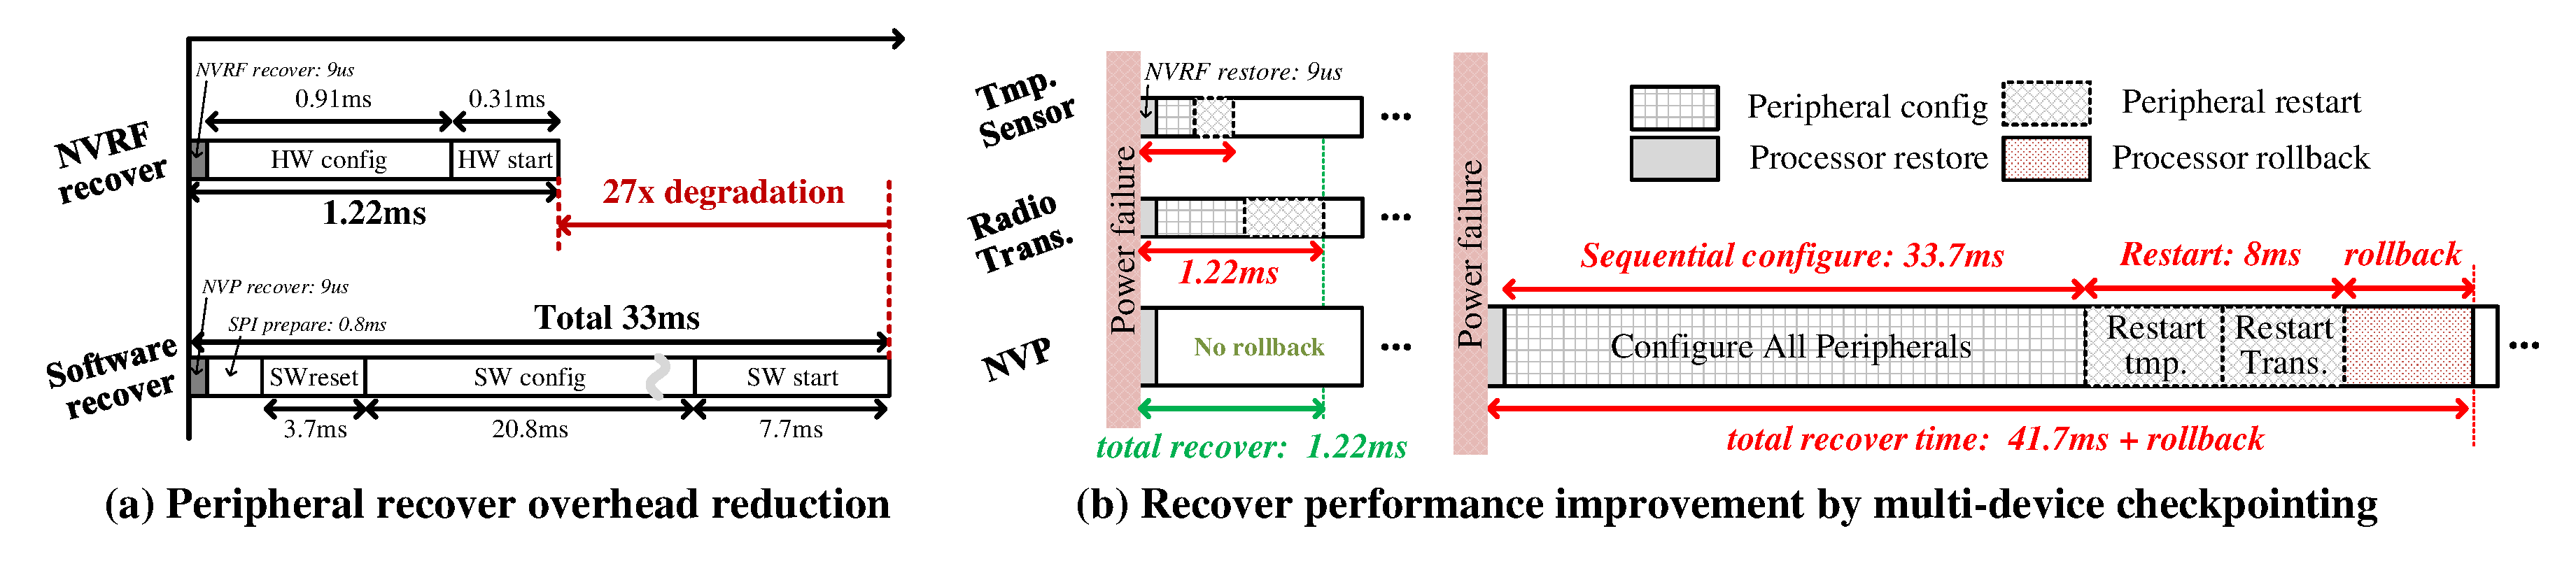
\includegraphics[width=1\textwidth]{Fig12_ImpCompare.pdf}
    %\vspace{-25pt}
    \caption{Recover overhead and task completeness comparison between REMARK and SDRB.}
    %%\vspace{-5pt}
    \label{fig:ImpCompare}
\end{figure*}

\subsection{Overall Performance Evaluation} \label{sec:implOverall}
%\vspace{-5pt}
%
The improvement in recovery performance leads to better overall system performance. 
A \emph{`bridge-monitoring'} application, a pure transmission application, and a pure sensing application are used to evaluate the overall performance improvement.
\emph{`bridge-monitoring'} is a data collecting application which contains both sensing and transmission tasks. 
These tasks are repeated periodically.
The work flow of \emph{`bridge-monitoring'} is shown in Fig.~\ref{fig:ImpOverall} (a).
The power trace is a Wi-Fi power profile, whose average power is $93.3\mu W$.
NVnode starts to work, when the capacitor is charged to $5V$.
The system fails and the capacitor gets recharged when the voltage of capacitor falls below $1.2V$.

The benchmarks are executed for $2$ minutes with REMARK and SDRB.
Fig.~\ref{fig:ImpOverall} (b) compares the task completion efficiency.
For the benchmarks with pure transmission and sensing tasks, REMARK achieves $5.7\times$ and $5.6\times$ efficiency improvements.
For the ‘bridgemonitoring’ benchmark, REMARK completes $13\times$ more data collection and transmission tasks than SDRB.
This is because the latter contains more peripherals where the performance of SDRB significantly deteriorates.
Due to the improvement in task completion efficiency, the energy consumption is also reduced accordingly. 

\begin{figure}[t]
    \centering
    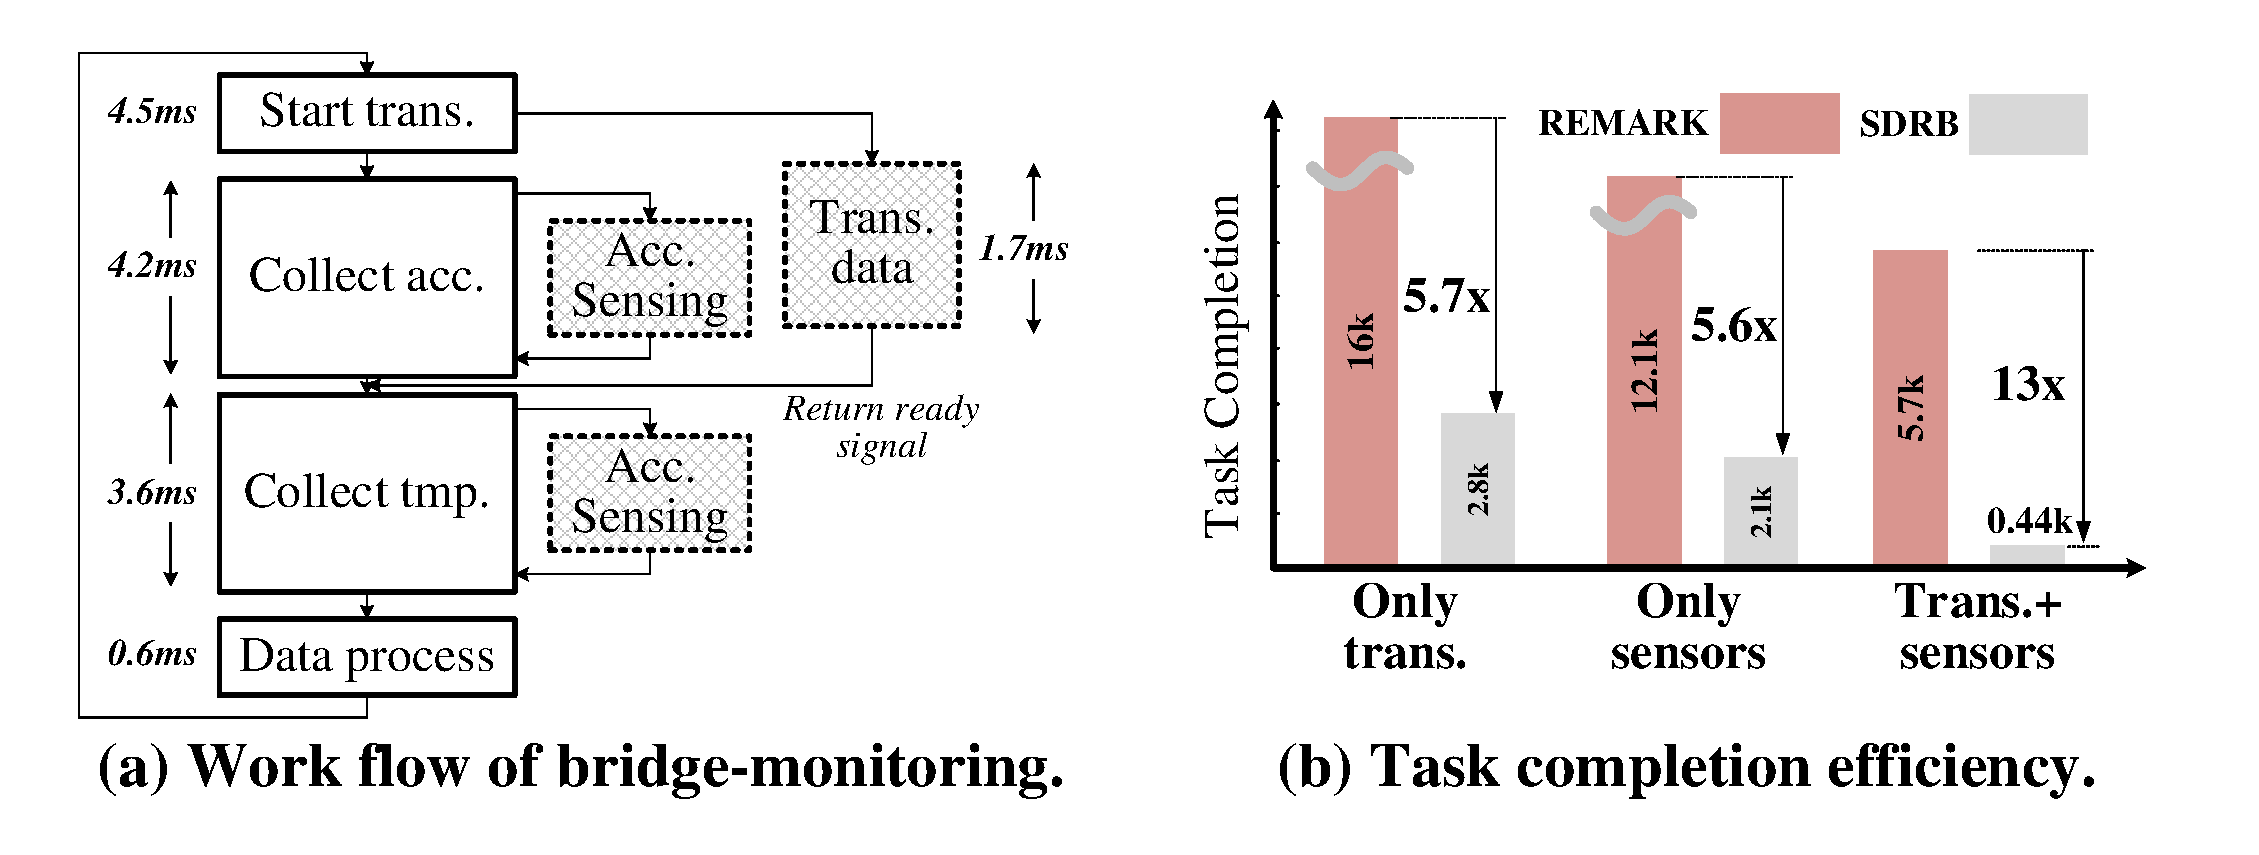
\includegraphics[width=0.5\textwidth]{Fig12_ImpOverall.pdf}
    %\vspace{-20pt}
    \caption{\emph{bridge-monitoring} application and task completeness comparison between REMARK and SDRB.}
    %\vspace{-5pt}
    \label{fig:ImpOverall}
    %\vspace{-0pt}
\end{figure}

\begin{comment}
%
\begin{figure}[t]
    \centering
    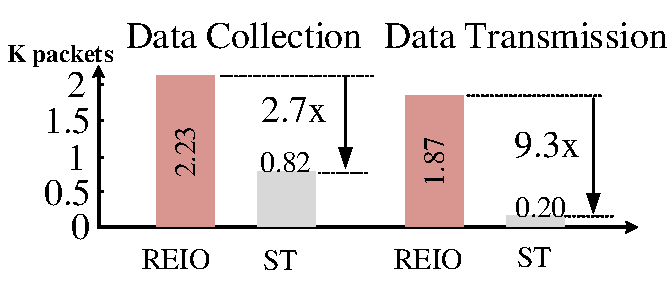
\includegraphics[width=0.3\textwidth]{Fig12_ImpRecover.pdf}
    %\vspace{-10pt}
    \caption{Performance comparison of REMARK and REMARK by executing \emph{bridge-monitoring} for $2$ minutes on NVnode.}
    \label{fig:ImpRecoverEvaluate}
    %\vspace{-0pt}
\end{figure}

\begin{comment}
{To decouple the effect of outage rates, Fig.}~\ref{fig:ImpRecoverEvaluate}{ (a) shows an example of a typical recover procedure after one power failure, where REMARK reduces the recovery overhead by 61.8\%.}
%Fig.~\ref{fig:ImpRecoverEvaluate}{ (c) shows the overhead breakdown of REMARK and QuickRecall. REMARK improves the validate execution time from total overheads.}
 
%\noindent$\bullet$
\textbf{Re-initialization overhead} 
        Compared with the \emph{`init-all'} strategy in QuickRecall, REMARK reduces the re-initialization overhead from 55\% to 11\% with the \emph{`init-used'} strategy.

\textbf{B/R overhead} 
        B/R overhead represents the backup/restore overhead. Using hardware B/R functions, REMARK incurs negligible B/R time overhead.
     
\textbf{Rollback overhead} 
        The rollback overhead is a random scaled overhead which depends on the position where power failure disrupts the program. REMARK is able to complete more tasks with comparable rollback overheads of QuickRecall.


In conclusion, \emph{REMARK guarantees the reliability of I/O and peripheral operations, and the data transmission/collection completeness is improved by $9.3\times$/$2.7\times$  compared with the existing state-of-the-art software recovery strategies}.

%
\begin{figure}[t]
    \centering
    \includegraphics[width=0.5\textwidth]{Fig13_ImpOverheadDeadlock.pdf}
    %\vspace{-20pt}
    \caption{{Overhead and resilience analysis. (a) the overhead of wrapper code. (b) a micro case study of the worst case when the outage rate is too high. (c) a sweep analysis of recovery overhead with power failure rates.}}
    \label{fig:ImpOverheadDeadlock}
    %\vspace{5}
\end{figure}
\end{comment}
\vspace{-0pt}
\section{Evaluation and Analysis} \label{sec:evaluation}
\vspace{-5pt}
%
In addition to the real chip evaluation, we also want to investigate the impact of design parameters in REMARK.
To explore larger design space, we develop a simulator, \emph{NVnodeSim} to gain more insights in designing TPC system.
In this section, we first present the simulator in Sec.~\ref{sec:expSettings}. 
Then, we tune the simulator to different settings and evaluate it with more general benchmarks to show how different design options affect the system performance in Sec.~\ref{sec:expEvaluation} and ~\ref{sec:expParaAnalysis}. 
Based on the observations, we summarize three design rules in Sec~\ref{sec:expRules}. 

%\vspace{-5pt} 
\subsection{Experiment Settings} \label{sec:expSettings}
\vspace{-5pt}
% Simulator
The inputs of NVnodeSim are power traces and benchmark profiles.
The power traces are solar power data from an open source database~\cite{midc2015solar}.
The benchmarks consist of three kinds of operations as shown in Table~\ref{tab:benchmarks}.
All parameters are extracted from datasheets or the cycle-accurate processor simulator Keil C.
Three common computing tasks for IoT are adopted.
Two I/O interfaces and five peripherals are also used, including sensors, transceivers, and an off-chip memory.
%We construct sensor node benchmarks by combining different computation operations, I/O interface and peripherals.

\begin{table}[t]
\begin{center}
    \vspace{-5pt}
\caption{Benchmarks: compute, I/O and peri. oper.}  \label{tab:benchmarks}
    \vspace{-5pt}
\Fsize{8}
\renewcommand{\arraystretch}{1.5}

% Computing Operations Table
%\begin{tabular*}{9cm}{@{\extracolsep{\fill}}Ic|cIc|cIc|cI}
\begin{tabular}{Im{1.15cm}<{\centering}|m{0.85cm}<{\centering}Im{1.15cm}<{\centering}|m{0.8cm}<{\centering}Im{1.15cm}<{\centering}|m{0.85cm}<{\centering}I}
    \Xhline{1.2pt}
    compute operation       & time /cycles          & compute operation      & time /cycles          & compute operation       & time /cycles           \\
    \Xhline{1.2pt}
    crc16                & $122$                   & rsa                   & $409$       & fft16                  & $275$                  \\
    \Xhline{1.2pt}
\end{tabular}

% I/O Operations Table
%\begin{tabular*}{9cm}{@{\extracolsep{\fill}}Ic|c|c|cI}
\begin{tabular}{Im{1.4cm}<{\centering}|c|c|m{1.9cm}<{\centering}I}
    \Xhline{1.2pt}
    I/O bus             & init time/cycles          & read time/cycles               & write time/cycles            \\
    \Xhline{1.2pt}
    I2C                 & $403$                         & $270 + 90 \times N$        & $180 + 90 \times N\tnote{*}$        \\
    \Xhline{1pt}
    SPI                 & $171$                         & $320 + 80 \times N$         & $320 + 80 \times N$        \\
    \Xhline{1.2pt}
\end{tabular}

% Peripherals Table
%\begin{tabular*}{9cm}{@{\extracolsep{\fill}}Ic|c|c|c|cI}
\begin{tabular}{Ic|c|c|c|cI}
    \Xhline{1.2pt}
    Peripheral                  & Chip                  & init./ms          & I/O bus       & exec time/ms    \\
    \Xhline{1.2pt}
    ZigBee                       & ML7266             & 531        & SPI        & $5.7 + 0.14 \times N$    \\
    %\Xhline{1pt}
    %Bluetooth                  & CC2540              & 1101        & SPI       & $1.2 + 0.37 \times N$    \\
    %\Xhline{1pt}
    %Light Sensor              & NOA1305          & 1451        & I2C       & 0.644    \\
    \Xhline{1pt}
    Acc. Sensor           & LIS331DLH       & 2391        & I2C       & 0.451    \\
    \Xhline{1pt}
    Image Sensor             & LUPA1300        & 14,952     & I2C       & 118.0    \\
    \Xhline{1pt}
    Tmp. Sensor               & TMP101           & 566          & I2C       & 0.283    \\
    \Xhline{1pt}
    FeRAM Mem            & FM25V20          &  76           & SPI        & --    \\
    \Xhline{1.2pt}
\end{tabular}

%\begin{tablenotes}
%    \footnotesize
%    \item[*] The number of transmited bytes.
%\end{tablenotes}

    \vspace{-10pt}
\end{center}
%\end{threeparttable}
\end{table} 

%
To validate the accuracy of NVnodeSim, Table~\ref{tab:SimValidateResults} compares the task execution time between NVnode and NVnodeSim.
It shows that NVnodeSim provides reasonable accuracy for architecture-level exploration.

\begin{table}[t]
\begin{center}
\vspace{-10pt}
\caption{Accuracy evaluation of NVnodeSim.} \label{tab:SimValidateResults}
\vspace{-5pt}
\Fsize{8}
\renewcommand{\arraystretch}{1.5}
%\setlength{\tabcolsep}{1pt}
\begin{tabular}{Im{1.37cm}<{\centering}Ic|m{0.89cm}Ic|m{0.99cm}IcI}
    \Xhline{1.2pt}
    \multirow{2}{*}{Benchmarks}     & \multicolumn{2}{cI}{Failure Times}       & \multicolumn{3}{cI}{Execution Time/ms} \\
                                                            \Xcline{2-6}{1pt}
                                                            & NVnode               & Sim                             & NVnode                & Sim                      & Error         \\
    \Xhline{1pt}
    RSA                                                & 3                           & 3                                 & 3.560                    & 3.512                   & -1.35\%        \\
    \Xhline{1pt}
    CRC                                                & 1                          & 1                                 & 1.316                    & 1.309                   & -0.53\%        \\
    \Xhline{1pt}
    MemLS                                           & 12                        & 11                               & 12.05                    & 11.99                   & -0.49\%        \\
    \Xhline{1pt}
    Sense                                               & 42                        & 42                               & 42.95                    & 42.38                   & -1.33\%        \\
    \Xhline{1.2pt}
\end{tabular}
\end{center}
    \vspace{-10pt}
\end{table} 

%\vspace{-5pt}
\subsection{Evaluation with Multiple Benchmarks} \label{sec:expEvaluation}
\vspace{-5pt}
% 
We further evaluate the performance of REMARK with ten additional benchmarks on the simulator.
Fig.~\ref{fig:I/OPerformance} (a) shows the recovery overhead distribution under ten benchmarks.
On average, REMARK reduces total overhead by 64\% compared with SDRB.
Fig.~\ref{fig:I/OPerformance} (b) shows that, the overhead of SDRB rises rapidly when multiple peripherals are included in the program.
This is because the re-initialization overhead grows rapidly.
The system even falls into deadlock when the re-initialization overhead is too large to complete during power failure intervals.
Thanks to the efficient \emph{`init-used'} strategy, the re-initialization overhead of REMARK stays modest.
From the experiment, we can see that \emph{REMARK can recover the system with multiple peripherals more efficiently and reliably}.

%
\begin{figure*}[t]
    \centering
    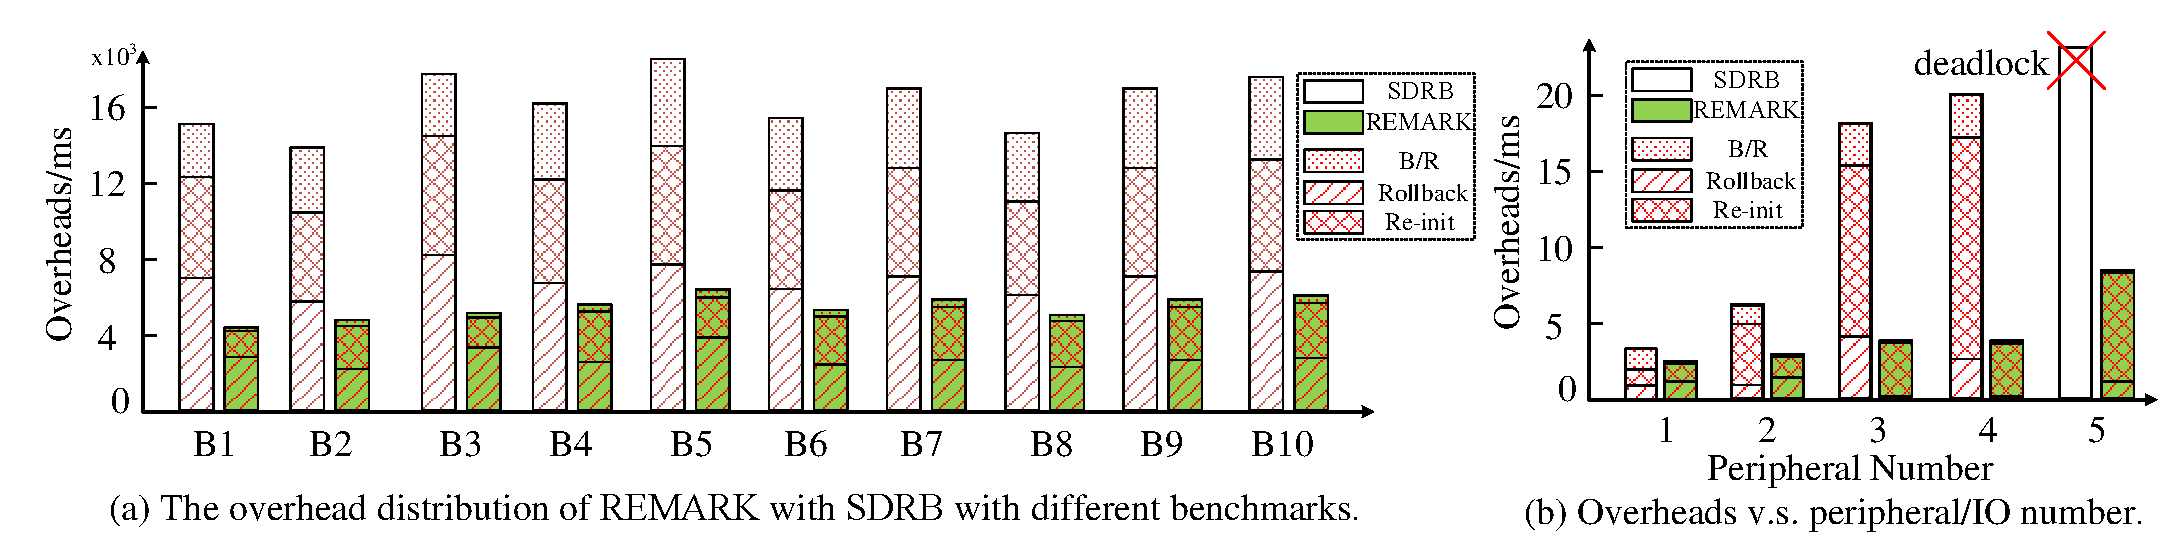
\includegraphics[width=0.9\textwidth]{Fig16_ExpIOPerformance.pdf}
    \vspace{-5pt}
    \caption{Recover overheads comparison between REMARK and SDRB.}
    \vspace{-0pt}
    \label{fig:I/OPerformance}
\end{figure*}

%\vspace{-5pt}
\subsection{Analysis the Peripheral Related Factors} \label{sec:expParaAnalysis}
\vspace{-5pt}
%
An important observation in Fig.~\ref{fig:I/OPerformance} is that the re-initialization and rollback overheads dominate the recovery overhead of REMARK.
These overheads are caused by peripheral disruptions.
The operation distribution in the program profile has a direct effect on peripheral disruptions.
Therefore, we explore the impact of three distribution factors of I/O and peripheral operations as below to gain insights on TPC system design.

%
\begin{figure}[t]
    \centering
    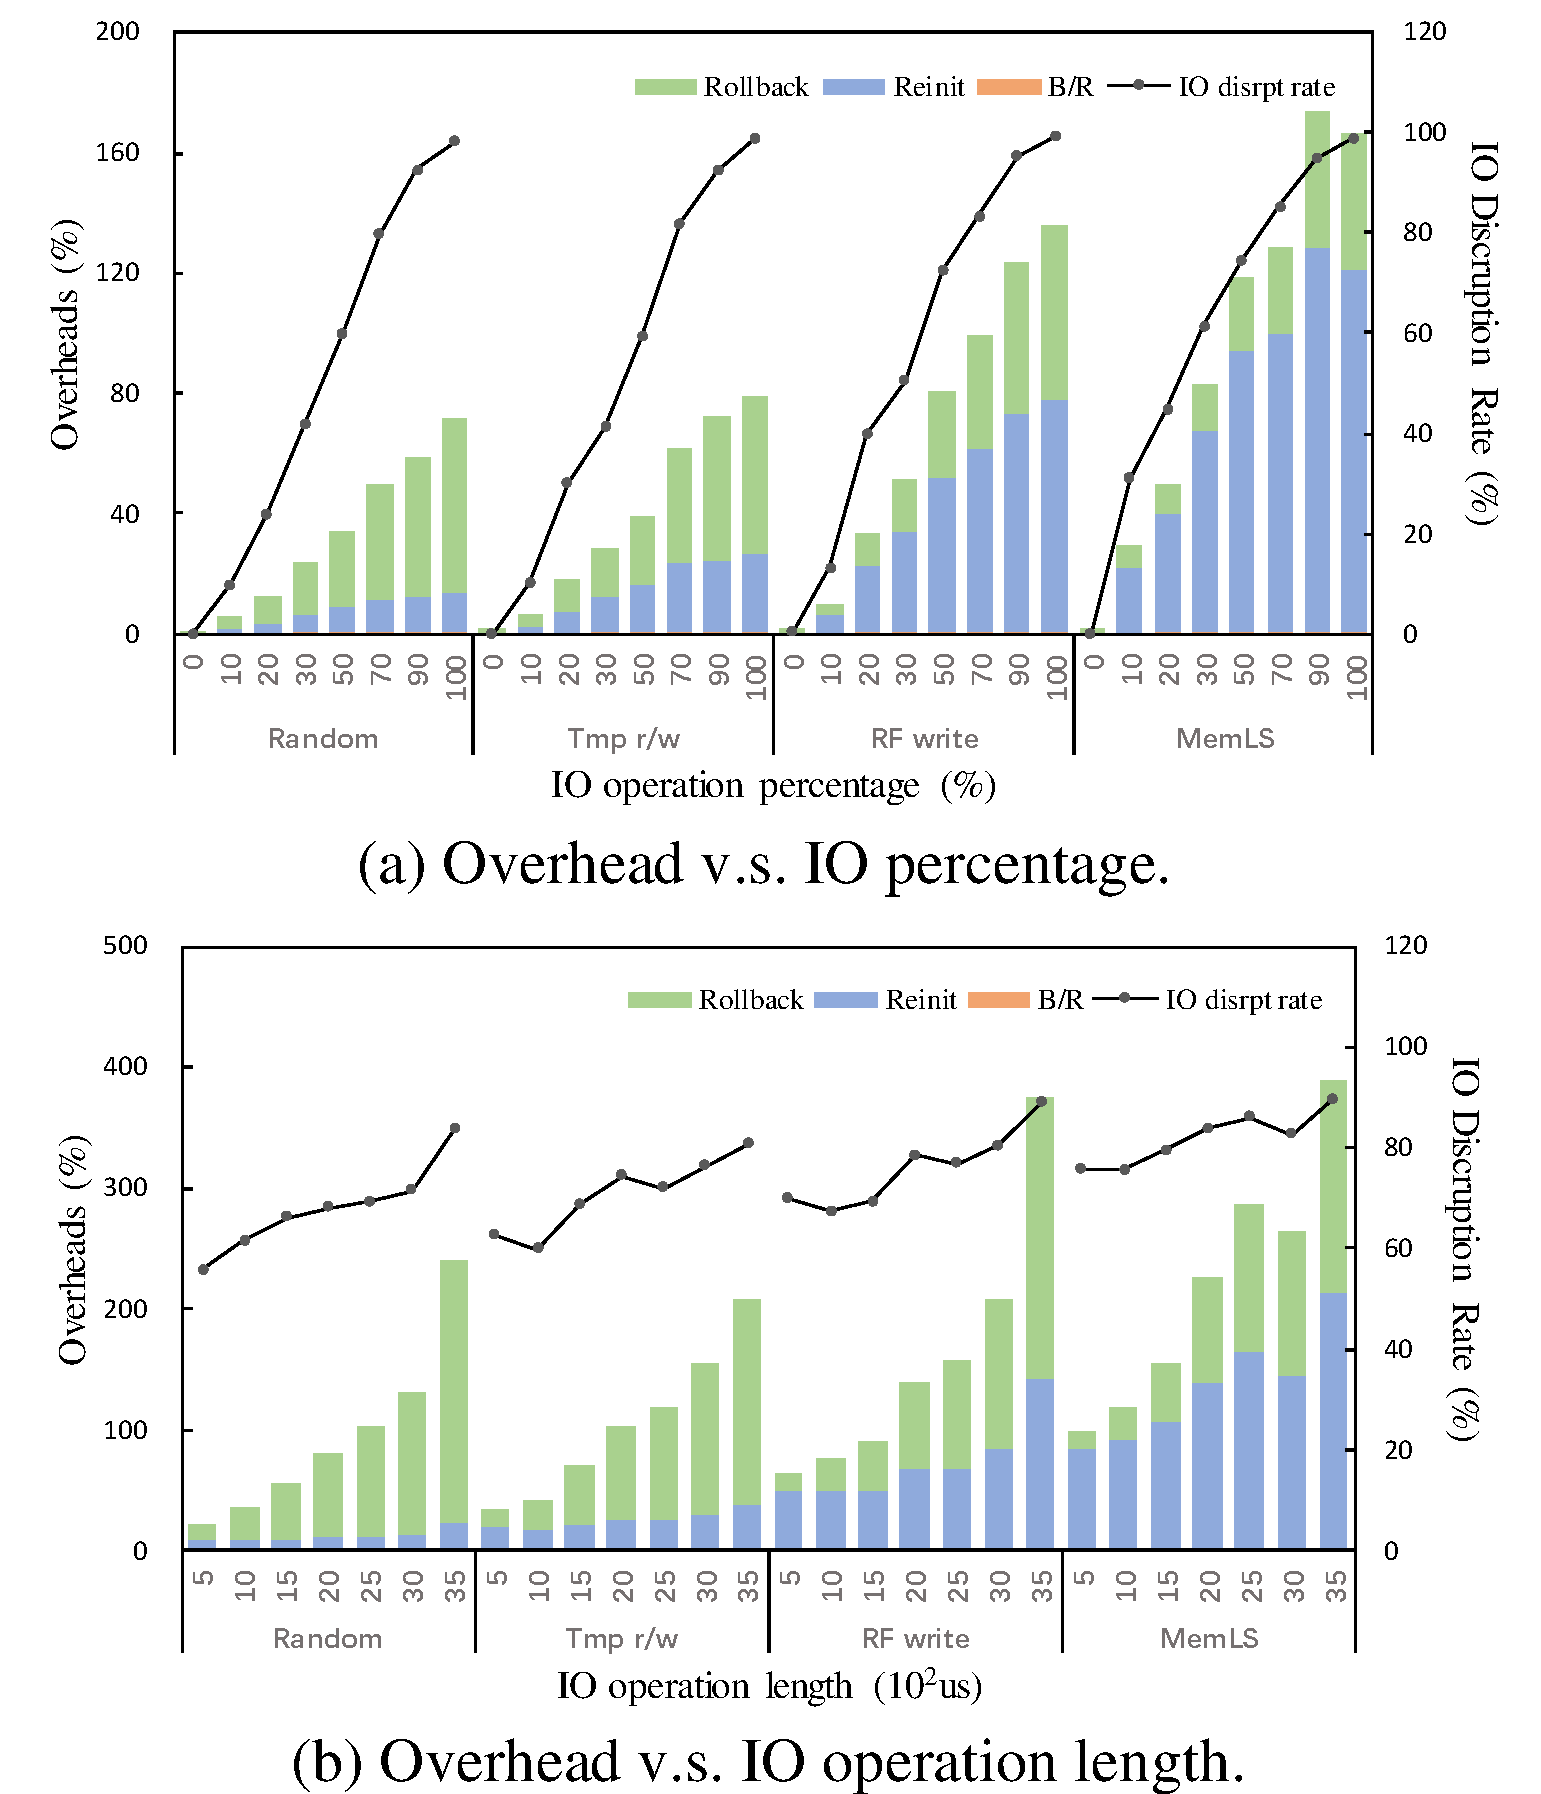
\includegraphics[width=0.4\textwidth]{Fig15_ExpPeriOperDistribute.pdf}
    \vspace{-5pt}
    \caption{{The performance overheads with various peripheral operation percentage and length.}}
    \vspace{-5pt}
    \label{fig:ExpPeriOperDistribute}
\end{figure}

\vspace{5pt}
\noindent\textbf{Peripheral Operation Percentage.} \\
Fig.~\ref{fig:ExpPeriOperDistribute} (a) shows the overheads and the failure times using benchmarks containing different peripheral operation percentages.
When more peripheral operations are used in a benchmark, power failures are more likely to cause peripheral disruptions.
According to the results, when the percentage increases, the total overhead increases slower than linear trend.
The reason is that recovering peripherals introduces more peripheral operations which increase its actual percentage compared with the original program.
Therefore, when a benchmark contains more than $70\%$ peripheral operations, the actual percentage approaches saturation and the total overhead grows slowly.

\vspace{5pt}
\noindent\textbf{Peripheral Operation Length.} \\
The length of each I/O operation affects the rollback distance during recovery.
Fig.~\ref{fig:ExpPeriOperDistribute} (b) shows the effect of lengths on the peripheral disruption times and the recovery overheads.
Rollback overhead increases when the length of peripheral operation increases from $0.5ms$ to $3.5ms$.
This is because longer peripheral operations may cause higher rollback distance.
Therefore, \emph{shorten the length of each peripheral operation can reduce the overhead of single recovery}.

\begin{comment}
% length v.s. the disruption times
Fig.~\ref{fig:ExpPeriOperDistribute} (b) shows that more peripheral disruptions take place when the length grows.
In statistics analysis, the peripheral disruption rate is affected only by peripheral operation percentage.
However, longer peripheral recover procedure increases this percentage, causes significant avalanche effects and leads to higher peripheral disruption rate.
In conclusion, \emph{the longer I/O operation length also increases the I/O disruption probability because of the avalanche effect}.
\end{comment}

\vspace{5pt}
\noindent\textbf{Overlap of I/O and Peripheral Operations.} \\
%
Since the processor and peripherals operate in parallel, the interaction among these devices also affects the performance of REMARK.
This part explores the impact of the overlap between I/O and peripheral operations.

In a wireless sensor node, I/O operations are executed by the processor, including off-chip memory accesses, sensor configurations, etc.
Peripheral operations are executed on peripherals, including sensing and data transmission tasks.
In such a system, the total recovery overhead of the system is determined by the largest overhead either on the processor or the peripheral.
Table~\ref{tab:OverheadPeriTask} shows the recovery overhead under different overlap ratios, where I/O/Peri. overlap is the overlap percentage of the I/O and peripheral operations.
The I/O/Peri. overlap ranges from $0$ to $100\%$ in two different benchmarks (sensing and data transmission). 
The breakdown of the recovery overhead of processor and peripherals are shown.
The stall time represent that the processor waits for the peripherals.
Overhead reduction shows how much reduction is achieved when there are more overlaps compared with the program with no overlap.
Results show that, the overhead decreases as much as $36.5\%$ when the overlap percentage increases.

Since most of sensor nodes work in a periodical way, overlapping I/O operations of previous loops with peripheral operations in current loop could be an effective solution to avoid large recovery overhead.
Therefore, \emph{with REMARK, software designer should overlap I/O and peripheral operations as much as possible to reduce the stall time of recovery process}.

\begin{table}[t]
\begin{center}
    \vspace{-5pt}
\caption{Overheads with different overlap percentages.} \label{tab:OverheadPeriTask}
    \vspace{-5pt}
\Fsize{8}
\renewcommand{\arraystretch}{1.5}
\begin{tabular}{Im{2.1cm}Ic|c|cIc|c|cI}%33.8 %40.3
    \Xhline{1.2pt}
    Benchmarks                                    & \multicolumn{3}{cI}{Sensing}                  & \multicolumn{3}{cI}{Data Transmission} \\
    \Xhline{1pt}
    I/O/Peri. overlap                               & 0\%           & 50\%         & 100\%             & 0\%           & 50\%         & 100\%        \\
    \Xhline{1pt}
    proc. overhead /\%                          & 44.9           & 43.6           & 43.4                & 43.4          & 42.7          & 41.7        \\
    \Xhline{1pt}
    peri. overhead /\%                           & 18.4            & 16.0           & 18.3                & 80.9          & 74.8          & 74.2       \\
    \Xhline{1pt}
    stall time/\%                               & 18.4            & 10.8           & 6.1                  & 80.9          & 62.4          & 39.2       \\
    \Xhline{1pt}
    Total overhead /\%                         & 63.3           & 54.4           & 49.5                & 124.3        & 105.1         & 78.9       \\
    \Xhline{1pt}
    {Overhead Reduction/\%}                         & --           & {14.0}           & {21.8}               & --        & {15.4}         & {36.5}       \\
    \Xhline{1.2pt}
\end{tabular}
\end{center}
\vspace{-10pt}
\end{table} 

\subsection{Analysis Conclusion} \label{sec:expRules}
\vspace{-5pt}
%
The evaluation experiments show that REMARK is able to support the reliability and task progress of a TPC system with multiple peripherals.
According to these analysis, we summarize three design rules for performance-aware software:

\begin{itemize}
    \item \textbf{Smaller I/O percentage.} 
        Reduce I/O operations as much as possible in TPCs to avoid expensive recovery overhead.
 
    \item \textbf{Shorter I/O operation length.}  
        Shorter I/O operations have smaller overhead. It is benefit to split a long I/O operation into several shorter ones.
     
    \item \textbf{More overlap between I/O and peripheral operations.} 
        Overlapping parallel operations can remove the stall time of the recovery process. It is also benefit to overlap the sensing and transmission operations in different cycles.

\end{itemize}











\section{Related Work} \label{sec:related}
%%\vspace{-5pt}
%
To support the task progress under intermittent power supply, both software and hardware recovery mechanisms have been proposed to support automatic recovery of the processor.

%\vspace{5pt}
\noindent\textbf{Software Mechanism: Checkpointing.} \\
%
Checkpointing is a software based recovery mechanism for processors.
Checkpoints are placed in the program, where the processor state are stored into non-volatile memories.
By rolling back to these checkpoints, the processor can keep the task progress after power failure~\cite{Dong2011Hybrid, Ma2015Architecture}.
Bronevetsky et al. propose the application level checkpointing strategy on the shared memory systems to enhance the reliability~\cite{Bronevetsky2004Application}.
Mementos proposes the concept of transiently powered computer and presents a software processing strategy which transforms the general purpose programs into interruptible computations for the general hardware architecture with Flash memory~\cite{ransford2012mementos}.
Balsamo et al. propose Hibernus and Hibernus++ using FeRAM and an interrupt-based checkpointing solution to reduce the performance overhead~\cite{balsamo2015hibernus,Balsamo2016Hibernus++,Rodriguez2015Approaches}.
Jayakumar et al. design QuickRecall and em-Map to integrate FeRAM into main memory to reduce the backup data size and lower the failure voltage threshold~\cite{jayakumar2014quickrecall,jayakumar2015q}.
In addition to general purpose processor architectures, Mirhoseini et al. target the Application Specific Integrated Circuits (\emph{ASICs}) and propose Idetic and Chime with the help of control data flow graphs (\emph{CDFGs})~\cite{Mirhoseini2013Idetic,Mirhoseini2013Automated,Mirhoseini2016Chime}.

These schemes achieve continuous progress of processors with out peripherals.
Large rollback overhead may take place while recovering a multi-device system with these strategies. 

%\vspace{5pt}
\noindent\textbf{Hardware Mechanism: Non-volatile Processor.} \\
%
Besides the checkpointing mechanisms, researchers also provide solutions in hardware domain.
Non-volatile processor draws a lot of attention due to its ability to store the system state and data automatically in hardware.
The first processor chip designed by Wang et al. using FeRAM realizes the ability to backup and restore the processor state and data within $3\mu s$~\cite{wang20123us}.
Bartling et al. propose a non-volatile logic based Cortex-M0 chip with higher performance and lower leakages~\cite{Bartling2013An}.
Sakimura et al. from NEC propose the non-volatile magnetic flip-flops~\cite{Sakimura2009Nonvolatile} and a 20MHz non-volatile micro-controller with STT-RAM~\cite{Sakimura201410}.
Recently, Liu et al. propose an enhanced NVP based on ReRAM which has the highest integration level~\cite{liu2016a}.
In addition, Li et al. propose the non-volatile I/O (NVIO) enabling efficient automatic reconfiguration of  I/O interfaces~\cite{li2016hw}.

Compared with software checkpointing strategies, non-volatile devices enable state recovery with higher speed and fewer rollbacks.
However, these nonvolatile processors lack of flexibility on checkpointing and recovery which may cause inconsistency problems in a multi-device system.


%\vspace{5pt}
\noindent\textbf{Inconsistency and Program Partitioning.} \\
%
Researchers have noticed the problem of the inconsistency issues while rolling back a system with nonvolatile memories.
B. Lucia et al.~\cite{Lucia2015} discover and model the data inconsistency problem caused by improper rollbacks after power failures.
After that, more works~\cite{van2016intermittent}, ~\cite{colin2016chain}, ~\cite{Xie2015} analyze the scenarios of checkpoint recoveries and propose careful checkpointing strategies to ensure the correctness of all checkpoints.
Recently, an energy-interference-free debugger for intermittent powered systems is proposed by A. Colin et al. to provide a more reliable and convenient debugging platform~\cite{Colin2016An}.
However, reliabliliy and efficiency challenges still exist when adopting NVP in a TPC system with multiple peripherals and interrupts.

%These works analyzes the transactional program in a TPC system and proposes proper program partitioning methods to avoid sematics issues caused by inconsistency.
%However, the consistency of the processor and the multiple peripherals raises new challenges.
%Therefore, REMARK is proposed target on the efficiency and reliability challenges in the recovery of multi-device TPC systems.

%\section{Future Work} \label{sec:future}
%
\section{Conclusion} \label{sec:conclution}
%
This paper proposes REMARK, a \underline{R}eliable and \underline{E}fficient \underline{M}ultitask Recovery Fr\underline{A}mewo\underline{RK}, which realizes reliable and efficient TPC recovery.
REMARK provides an automatic and efficient peripheral recover hardware architecture supporting the system with multiple peripherals.
Moreover, a new checkpointing strategy for the multi-device system is also provided to avoid the inconsistency issues between different devices and incurs the lowest rollback overhead.
A REMARK-enabled NVP is fabricated and evaluated, which demonstrates that REMARK enables reliable data transmission with $13\times$ completeness improvements compared with state-of-the-art. 
In conclusion, REMARK implements a critical component that existing NVP solutions are missing and will greatly improve the applicability of TPCs in the IoT era.


%\section{Acknowledgement} \ref{sec: acknowledgement}
% 
%\end{spacing}

%%%%%%% -- PAPER CONTENT ENDS -- %%%%%%%%

%%%%%%%%% -- BIB STYLE AND FILE -- %%%%%%%%
\bibliographystyle{ieeetr}
\bibliography{references}
%%%%%%%%%%%%%%%%%%%%%%%%%%%%%%%%%%%%

\end{document}
